\documentclass[12pt,twoside,notitlepage]{report}

\usepackage{a4}
\usepackage{verbatim}
\usepackage{graphicx}
\usepackage{listings}

\raggedbottom                           % try to avoid widows and orphans
\setlength{\topskip}{1\topskip plus 7\baselineskip}
\sloppy
\clubpenalty1000%
\widowpenalty1000%

\addtolength{\oddsidemargin}{6mm}       % adjust margins
\addtolength{\evensidemargin}{-8mm}

\renewcommand{\baselinestretch}{1.1}    % adjust line spacing to make
                                        % more readable

\setlength{\parskip}{1.3ex plus 0.2ex minus 0.2ex}
\setlength{\parindent}{0pt}

\setcounter{secnumdepth}{5}
\setcounter{tocdepth}{5}

\lstset{
  basicstyle=\small,
  language={[Sharp]C},
  tabsize=4,
  numbers=left,
  frame=none,
  frameround=tfft
}


\begin{document}


\bibliographystyle{plain}


%%%%%%%%%%%%%%%%%%%%%%%%%%%%%%%%%%%%%%%%%%%%%%%%%%%%%%%%%%%%%%%%%%%%%%%%
% Title


\pagestyle{empty}

\hfill{\LARGE \bf David Srbeck\'y}

\vspace*{60mm}
\begin{center}
\Huge
{\bf .NET Decompiler} \\
\vspace*{5mm}
Part II of the Computer Science Tripos \\
\vspace*{5mm}
Jesus College \\
\vspace*{5mm}
May 16, 2008
\end{center}

\cleardoublepage

%%%%%%%%%%%%%%%%%%%%%%%%%%%%%%%%%%%%%%%%%%%%%%%%%%%%%%%%%%%%%%%%%%%%%%%%%%%%%%
% Proforma, table of contents and list of figures

\setcounter{page}{1}
\pagenumbering{roman}
\pagestyle{plain}

\section*{Proforma}

{\large
\begin{tabular}{ll}
Name:               & \bf David Srbeck\'y                       \\
College:            & \bf Jesus College                         \\
Project Title:      & \bf .NET Decompiler                       \\
Examination:        & \bf Part II of the Computer Science Tripos, 2008        \\
Word Count:         & \bf 11949\footnotemark[1]         \\
Project Originator: & David Srbeck\'y                   \\
Supervisor:         & Alan Mycroft                      \\ 
\end{tabular}
}
\footnotetext[1]{This word count was computed
by {\tt detex diss.tex | tr -cd '0-9A-Za-z $\tt\backslash$n' | wc -w}
}
\stepcounter{footnote}

\subsection*{Original Aim of the Project}

The aim of this project was to create a .NET decompiler.
That is, to create a program that translates .NET executables 
back to C\# source code.
%This is essentially the opposite of a compiler.

The concrete requirement was to decompile a 
quick-sort algorithm.  Given an implementation of a quick-sort 
algorithm in executable form, the decompiler was required
to re-create semantically equivalent C\# source code.  
Although allowed to be rather cryptic, the generated source code 
had to compile and work without any additional modifications.


\subsection*{Work Completed}

Implementation of the quick-sort algorithm decompiles successfully.
Many optimizations were implemented and perfected to the
point where the generated source code for the quick-sort 
algorithm is practically identical to the original%
\footnote{See pages \pageref{Original quick-sort} and \pageref{Decompiled quick-sort} in the evaluation chapter.}.
In particular, the source code compiles back to identical .NET CLR code.

Further challenges were sought in more complex programs.
The decompiler deals with several issues which did not
occur in the quick-sort algorithm.  It also implements some
optimizations that are only applicable to the more complex programs.


\subsection*{Special Difficulties}

None.
 
\newpage
\section*{Declaration}

I, David Srbeck\'y of Jesus College, being a candidate for Part II of the Computer
Science Tripos, hereby declare
that this dissertation and the work described in it are my own work,
unaided except as may be specified below, and that the dissertation
does not contain material that has already been used to any substantial
extent for a comparable purpose.

\bigskip
\leftline{Signed}

\medskip
\leftline{Date}

\cleardoublepage

\tableofcontents

\listoffigures


\cleardoublepage        % just to make sure before the page numbering
                        % is changed

\setcounter{page}{1}
\pagenumbering{arabic}
\pagestyle{headings}

%%%%%%%%%%%%%%%%%%%%%%%%%%%%%%%%%%%%%%%%%%%%%%%%%%%%%%%%%%%%%%%%%%%%%%%%%%%%%%%
% 3 Pages
\chapter{Introduction}

\section{The goal of the project}
% Decompiler
% .NET

The goal of this project is to create a .NET decompiler.

Decompiler is a tool that translates machine code back to source
code.  That is, it does the opposite of a compiler -- it takes the 
executable file and it tries to recreate the original source code.

In general, decompilation can be extremely difficult or even impossible.
Therefore this project focuses on something slightly simpler -- 
decompilation of .NET executables.
The advantage of .NET executables is that they consist of processor 
independent bytecode which is easier to decompile then 
the traditional machine code because
the instructions are more high level and the code is less optimized.
The .NET executables also preserve a lot of metadata about the code like
type information and method names.

Note that despite its name, the \emph{.NET Framework} 
is unrelated to networking or the Internet and it is basically the
equivalent of \emph{Java Development Kit}.

To succeed, the produced decompiler is required to successfully decompile
a console implementation of a quick-sort algorithm back to C\# source code.


\section{Decompilation}

Decompilation is the opposite of compilation.  It takes the executable
file and attempts to recreate the original source code.
Despite of doing the reverse, decompilation is very similar to
compilation.  This is because both compilation and decompilation do
in essence that same thing -- translate program from one form to
other form and then optimize the final form.
Because of this, many analysis and optimizations used in compilation
are also applicable in decompilation.

Decompilation may not always be possible.  In particular,
self-modifying code is very problematic.

\section{Uses of decompilation}

\begin{itemize}
    \item Recovery of lost source code.
	\item Reverse engineering of programs that ship with no
	  source code.  This, however, might be a bit controversial use
	  due to legal issues.
	\item Interoperability.
	\item Security analysis of programs.
	\item Error correction or minor improvements.
	\item Porting of executable to other platform.
	\item Translation between languages.
      Source code in some obscure language can be compiled into an 
      executable which can in turn be decompiled into C\#.
    \item Debugging of deployed systems.  Deployed system
      might not ship with source code or it might be difficult
      to `link' it to the source code because it is optimized.
      Also note that it might not be acceptable to restart 
      the running system because the issue is not easily reproducible.
\end{itemize}

\section{The .NET Framework}
% Bytecode - stack-based, high-level
% JIT
% Much metadata
% Typesafe

The \emph{.NET Framework} is a general-purpose software development platform 
which is very similar to the \emph{Java Development Kit}.
It includes an extensive class library 
and, similarly to Java, it is based on a virtual machine model which
makes it platform independent.

To be platform independent the program is stored in form of bytecode
(also called Common Intermediate Language or \emph{IL}).
The bytecode instructions use the stack to pass data around rather then
registers.
The instructions are aware of the object-oriented programing
model and are more high level then traditional processor instructions.
For example, there is special instruction to allocate an object in memory,
to access a field of an object, to cast an object to a different type
and so on.

The byte code is translated to machine code of the 
target platform at run-time.  The code is just-in-time compiled rather then
interpreted.  This means that the first execution of a function will be slow
due to the translation overhead, but the subsequent executions of the
same function will be very fast.

The .NET executables preserve a lot of information about the
structure of the program.  The complete structure of classes is
preserved including all the typing information.  The code is still
separated into distinct methods and the complete signatures of 
the methods are preserved -- that is, the executable includes
the method name, the parameters and the return type.

The virtual machine is intended to be type-safe. Before any code
is executed it is verified and code that has been successfully
verified is guaranteed to be type-safe.  For example, it is 
guaranteed not access unallocated memory.
However, the framework also provides some inherently unsafe
instructions.  This allows support for languages like C++, but
it also means that some parts of the program will be unverifiable.
Unverifiable code may or may not be allowed to execute depending
on the local security policy.

In general, any programming language can be compiled to \emph{.NET} and 
there are already dozens, if not hundreds, of compliers in existence.
The most commonly used language is \emph{C\#}.


\section{Scope of the project}

The \emph{.NET Framework} is mature comprehensive platform and handling
all of its features is out the scope of the project.  Therefore, it is
necessary to state which features should be supported and which
should not.

The decompiler was specified to at least handle all the features required
to decompile the quick-sort algorithm.  This includes integer arithmetic,
array operations, conditional statements, loops and system method calls.

The decompiler will not support so-called unverifiable instructions -- 
for example, pointer arithmetic and access to arbitrary memory locations.
These operations are usually used only for
interoperability with native code (code not running under the .NET 
virtual machine).  As such, these instructions
are relatively rare and do not even occur in many programs at all.

Generics also will not be supported.  They were introduced in the
second version of the Framework and many programs still do not make any
use of them.  The generics also probably does not provide any
theoretical challenge for the decompilation.  It just involves handing
of more bytecodes and more special cases of the existing bytecodes.

\section{Previous work}

Decompilers are in existence nearly as long as compilers.
The very first decompiler was written by Joel Donnelly in 1960 
under the supervision of Professor Maurice Halstead.
Initially, decompilers were created to aid in the program 
conversion process from second to third generation computers.
Decompilers were actively developed over the following
years and were used for variety of applications.

Probably the best know and most influential research paper
is \emph{Cristina Cifuentes' PhD Thesis ``Reverse Compilation 
Techniques'', 1994}.  As part of the paper Cristina
created a prototype \emph{dcc} which translates Intel i80286
machine code into C using various data and control flow
analysis techniques.

The introduction of virtual machines made decompilation
more feasible then ever (e.g.\ \emph{Java Virtual Machine} or
\emph{.NET Framework Runtime}).

There are already several closed-source .NET decompilers
in existence.  The most known one is probably
Lutz Roeder's \emph{Reflector for .NET}.

% Cristina 
% Current .NET Decompilers

%%%%%%%%%%%%%%%%%%%%%%%%%%%%%%%%%%%%%%%%%%%%%%%%%%%%%%%%%%%%%%%%%%%%%%%%%%%%%%%
% 12 Pages
\cleardoublepage
\chapter{Preparation}

This chapter explains the general idea behind the decompilation
process.  The implementation chapter then explains how these
methods were implemented and what measures were taken
to ensure the correctness of the produced output.

\section{Overview of the decompilation process}
% Read metadata
% Starting point
% Translating bytecodes into C# expressions;  
%   High-level;  Stack-Based;  Conditional gotos
% Dataflow analysis; inlining
% Control flow analysis (interesting)
% Suggar

The first step is to read and disassemble the \emph{.NET} executable files.
There is an open-source library called \emph{Cecil} which was created exactly
for this purpose.   It loads the whole executable into memory and then
it provides simple object-oriented API to access the content of the executable.
Using this library, the access to the executable is straightforward.

It is worth noting the wealth of information we are starting with.
The \emph{.NET} executables contain quite high-level representation
of the program.  Complete typing information is still present -- 
we have access to all the classes including the fields and methods.
The types and names are also preserved.
The bytecode is stored on per-method basis and even the local variables
used in the method body are still explicitly represented including the type.%
\footnote{However, the names of local variables are not preserved.}

Ultimately, the challenge is to translate the bytecode of a given
method to a C\# code.

For example, consider decompilation of following code:

\begin{verbatim}
// Load "Hello, world!" on top of the stack
ldstr "Hello, world!"
// Print the top of the stack to the console
call System.Console::WriteLine(string)
\end{verbatim}

We start by taking the bytecodes one by one and translate them
to C\# statements.  The bytecodes are quite high level so
the translation is usually straightforward.
The two bytecodes can thus be represented as the following 
two C\# statements (\verb|output1| and \verb|some_input| are just
dummy variables):

\begin{verbatim}
string output1 = "Hello, world!";
System.Console.WriteLine(some_input);
\end{verbatim}

The first major challenge of decompilation is data-flow
analysis.  In this example, we would analyze the stack
behavior and we would find that \verb|output1| is on the top
of the stack when \verb|WriteLine| is called.  Thus, we would get:

\begin{verbatim}
string output1 = "Hello, world!";
System.Console.WriteLine(output1);
\end{verbatim}

At this point the produced source code should already compile 
and work as intended.

The second major challenge of decompilation is control-flow 
analysis.  The use of control-flow analysis
is to replace \verb|goto| statements with high-level structures 
like loops and conditional statements.  This makes the produced 
source code much more easier to read and understand.

Finally, there are several sugarings that can be done to the code to
make it more readable -- for example, replacing \verb|i = i + 1| 
with the equivalent \verb|i++| or using rules of logic to 
simplify boolean expressions.

\section{Translating bytecodes into C\# expressions}
% One at a time
% Byte code is high level (methods, classes, bytecode commands)
% Types preserved (contrast with Java)

The first task is to convert naively the individual bytecodes into 
equivalent C\# expressions or statements.

This task is reasonably straightforward because the bytecodes 
are quite high level and are aware of the object-oriented
programming model.  For example, there are bytecodes
for integer addition, object creation, array access,
field access, object casting and so on; all of these trivially
translate to C\# expressions.

Any branching commands are also easy to handle because
C\# supports labels and \verb|goto|s.  Unconditional branches
are translated to \verb|goto| statements and conditional 
branches are translated to \verb|if (condition) goto Label;|.

C\# uses local variables for data transfer whereas bytecodes
use the stack.  This mismatch will be handled during the
data-flow analysis phase.  Until then, dummy variables
are used as placeholders.  For example, \verb|add| bytecode
would be translated to \verb|input1 + input2|.


\section{Data-flow analysis}
\subsection{Stack in .NET}
% Stack behavior
% Deterministic stack (tested - failed)

Bytecodes use a stack to pass data between consecutive 
instructions.  When a bytecode is executed, it pops its arguments
from the stack, it performs some operation on them and then
it pushes the result, if any, back to the stack.

The number of popped elements is fixed and known before execution time
- for example, any binary operation pops exactly two arguments and
a method call pops one element for each of its arguments.

Most bytecodes either push only one element on the stack or none at all.%
\footnote{There is one exception to this -- the `dup' instruction.
More on this later.}
This makes the data-flow analysis slightly simpler.

The framework imposes some useful restrictions with regards to
control-flow.  In theory, we could arrive at a given point in program
and depending on which execution path was taken, we could end up with
two completely different stacks.  This is not allowed.  Regardless
of the path taken, the stack must have the same number of elements in it.
The typing is also restricted -- if one execution path pushes an integer
on the stack, any other execution path must push an integer as well.

\subsection{Stack simulation}

Bytecodes use the stack to move data around, but there is no such stack
concept in C\#.  Therefore we need to use something that C\# does 
have -- local variables.

The transformation from stack to local variables is simpler then 
it might initially seem.  Basically, pushing something on the
stack means that we will need that value later on.  So in C\#,
we create a new temporary variable and store the value in it.
On the other hand, popping is a usage of the value.  So in C\#, 
we just reference the temporary variable that
holds the value we want.  The only difficult is to figure out
which temporary variable it is.

This is where the restrictions on the stack come handy -- we can
figure out what the state of the stack will be at any given point.
That is, we do not know what the value will be, but we do know
who pushed the value on the stack and what the type of the value is.
For example, after executing the following code
\begin{verbatim}
IL_01: ldstr "Hello''
IL_02: ldstr "world''
\end{verbatim}
we know that there will be exactly two values on the stack -- 
the first one pushed by bytecode labeled \verb|IL_01| and the 
second one pushed by bytecode labeled \verb|IL_02|.  Both of
them of are of type \verb|String|.  Let's say that the state
of the stack is \{\verb|IL_01|, \verb|IL_02|\}.

Now, let us pop value from the stack by calling 
\verb|System.Console.WriteLine|.  This method takes one
\verb|String| argument.  Just before the method is called
the state of the stack is \{\verb|IL_01|, \verb|IL_02|\}.
Therefore the value allocated by \verb|IL_02| is popped 
from the stack and we are left with \{\verb|IL_01|\}.  
Furthermore, we know which temporary local variable to
use in the method call -- the one that stores the value
pushed by \verb|IL_02|.

Let us call \verb|System.Console.WriteLine| again to completely
empty the stack and let us see what the produced C\# source code
would look like (the comments show the state of the stack 
between the individual commands).
\begin{verbatim}
// {}
String temp_for_IL_01 = "Hello'';
// {IL_01}
String temp_for_IL_02 = "world'';
// {IL_01, IL_02}
System.Console.WriteLine(temp_for_IL_02);
// {IL_01}
System.Console.WriteLine(temp_for_IL_01);
// {}
\end{verbatim}

\subsection{The `dup' instruction}

In general, bytecodes push either one value on the stack or none at all.
There is only one exception to this -- the \verb|dup| instruction.
The purpose of this instruction is to duplicate the value on top of the
stack.  Fortunately, it does not break our model.  The only significance
of the \verb|dup| instruction is that the same value will be used twice -
that is, the temporary local variable will be referenced twice.

The \verb|dup| instruction, however, makes some future optimizations 
more difficult.

The \verb|dup| instruction is used relatively rarely and 
it usually just saves a few bytes of disk space.
Note that the \verb|dup| instruction could always be replaced
by store to a local variable and two loads.

The \verb|dup| instruction can be used in expression like 
\verb|this.a + this.a| -- the value \verb|this.a| is obtained
once, duplicated and then the duplicates are added.

\subsection{Control merge points}

This in essence the most complex part of data-flow analysis.
It is caused by the possibility of multiple execution paths.
There are two scenarios that branching can cause.

The nice scenario is when a value is pushed in one location and,
depending on the execution path, can be popped in two or more different
locations.  This translates well into the local variable model -
it simply means that the temporary local variable will be referenced
several times and there is nothing special we need to do.

The worse scenario is when a value can be pushed on the sack
in two or more different locations and then it is poped only in one locations.
Example of this would be 
\verb|Console.WriteLine(condition ? "true": "false")| -- 
depending on the value of the condition either ``true'' or 
``false'' is printed.  This code snippet compiles into bytecode
with two possible execution paths -- one in which ``true'' is pushed
on the stack and one in which ``false'' is pushed on the stack.
In both cases the value is poped only once when 
\verb|Console.WriteLine| is called.

This scenario does not work well with the local variable 
model.  Two values can be pushed on the stack and so two temporary 
local variables are created --  one holding ``true'' and 
one holding ``false''.
Depending on the execution path either of these can be on the
top of the stack when \verb|Console.WriteLine| is executed and 
therefore we do not know which temporary variable to use as the argument
for \verb|Console.WriteLine|.  It is impossible to know.

This can be resolved by creating yet another temporary variable
which will hold the actual argument for the \verb|Console.WriteLine|
call.  Depending on the execution path taken, one of the previous
variables needs to be copied into this one.
So the produced C\# source code would look like this:
\begin{verbatim}
String sigma;
if (condition) {
  String temp1 = "true";
  sigma = temp1;
} else {
  String temp2 = "false";
  sigma = temp2;
}
Console.WriteLine(sigma);
\end{verbatim}

Note that this is essentially the trick that is used to obtain
single static assignment (SSA) form of programs during compilation.

In reality, this happens extremely rarely and it is almost exclusively
caused by the C\# \verb|?| operator.

\subsection{In-lining expressions}
% Generally difficult, but here SSA-SR
% Validity considered - order, branching

The code produced so far contains many temporary variables.
These variables are often not necessary and can be 
optimized away.  For example, the code

\begin{verbatim}
string output1 = "Hello, world!";
System.Console.WriteLine(output1);
\end{verbatim}

can be simplified into a single line:

\begin{verbatim}
System.Console.WriteLine("Hello, world!");
\end{verbatim}

Doing this optimization makes the produced code much more readable.

In general, removing a local variable from a method is non-trivial.
However, these generated local variables are special -- they were generated
to remove the stack-based data-flow model.
This means that the local variables are assigned only once and are
read only once%
\footnote{With the exception of the `dup' instruction which is read twice
and thus needs to be handled specially.}
(corresponding to the push and pop operations respectively).

There are some safety issues with this optimization.
Even though we are sure that the local variable is assigned and read
only once, we need to make sure that doing the optimization will not
change the semantics of the program.  For example consider the 
following code:

\begin{verbatim}
string output1 = f();
string output2 = g();
System.Console.WriteLine(output2 + output1);
\end{verbatim}

The functions \verb|f| and \verb|g| may have side-effects and in this 
case \verb|f| is called first and then \verb|g| is called.
Optimizing the code would produce 
\begin{verbatim}
System.Console.WriteLine(g() + f());
\end{verbatim}
which calls the functions in the opposite order.

Being conservative, we will allow this optimization only if the
declaration of the variable immediately precedes its use.
In other words, the variable is declared and then immediately
used with no possible side-effects in between these.
Using this rule, the previous example can be optimized to
\begin{verbatim}
string output1 = f();
System.Console.WriteLine(g() + output1);
\end{verbatim}
but it can not be optimized further because the function 
\verb|g| is executed between the declaration of \verb|output1|
and its use.


\section{Control-flow analysis}
% Recovering high-level structures

The main point of control-flow analysis is to recover high-level
structures like loops and conditional blocks of code.
This is not necessary to produce semantically correct code,
but it does make the code much more readable compared to
only using \verb|goto| statements.  It is also
the most theoretically interesting part of the whole
decompilation process.

In general, \verb|goto|s can be always completely removed
by playing some `tricks' like duplicating code or adding
boolean flags.  However, as far as readability of the
code is concerned, this does more harm than good.
Therefore, we want to remove \verb|goto|s using the `natural'
way -- by recovering the high-level structures they represent
in the program.  Any \verb|goto|s that can not be removed
in such way are left in the program.

See figures \ref{IfThen}, \ref{IfThenElse} and \ref{Loop}
for examples of control-flow graphs.

\begin{figure}[tbh]
\centerline{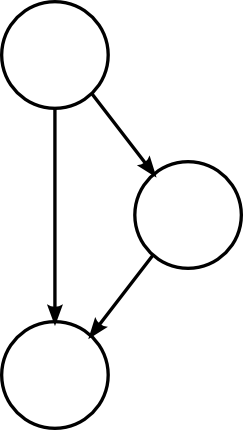
\includegraphics{figs/IfThen.png}}
\caption{\label{IfThen}Conditional statement (if-then)}
\end{figure}

\begin{figure}[tbh]
\centerline{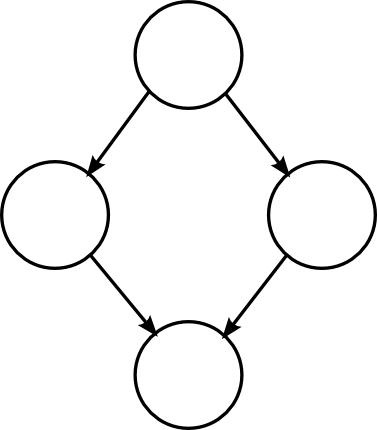
\includegraphics{figs/IfThenElse.png}}
\caption{\label{IfThenElse}Conditional statement (if-then-else)}
\end{figure}

\begin{figure}[tbh]
\centerline{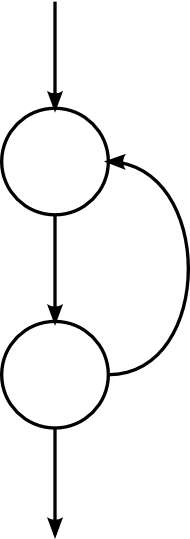
\includegraphics{figs/Loop.png}}
\caption{\label{Loop}Loop}
\end{figure}

\subsection{Finding loops}
% T1-T2 reduction
% Nested loops
% Goto=Continue=Break;  Multi-level break/continue

T1-T2 transformations are used to find loops.
These transformation are usually used to determine whether
a control flow graph is reducible or not, but
it turns out that they are suitable for finding loops as well.

If a control-flow graph is irreducible, it means that the
program can not be represented only using high-level structures.
That is, \verb|goto| statements are necessary to represent the
program.  This is undesirable since \verb|goto| statements
usually make the decompiled source code less readable.
See figure \ref{Ireducible} for the classical example
of irreducible control-flow graph.

\begin{figure}[tbh]
\centerline{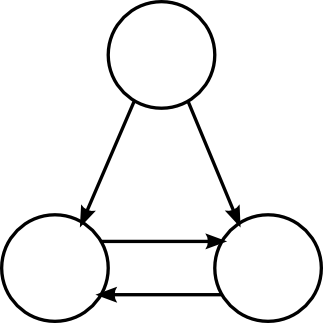
\includegraphics{figs/Ireducible.png}}
\caption{\label{Ireducible}Ireducible control-flow graph}
\end{figure}

If a control-flow graph is reducible, the program may or may not be
representable only using high-level structures.  That is,
\verb|goto| statements still may be necessary on some occasions.
For example, C\# has a \verb|break| statement which exits
the inner most loop, but it does not have any statement which
would exit multiple levels of loops.%
\footnote{This is language dependent.  
The Java language, for example, does provide such command.}
Therefore in such occasion we have to use the \verb|goto| statement.

The algorithm works by taking the initial control-flow graph
and then repeatedly applying simplifying transformations to it.  
As we can see from the name, the algorithm consists of two
transformations called T1 and T2.
If the graph is reducible, the algorithm will eventually simplify
the graph to only a single node.  If the graph is not reducible,
we will end up with multiple nodes and no more transformations
that can be performed.

Both of the transformations look for a specific pattern in
the graph and then replace the pattern with something simpler.

See figure \ref{T1T2} for a diagram showing the T1 and T2 transformations.

\begin{figure}[tbh]
\centerline{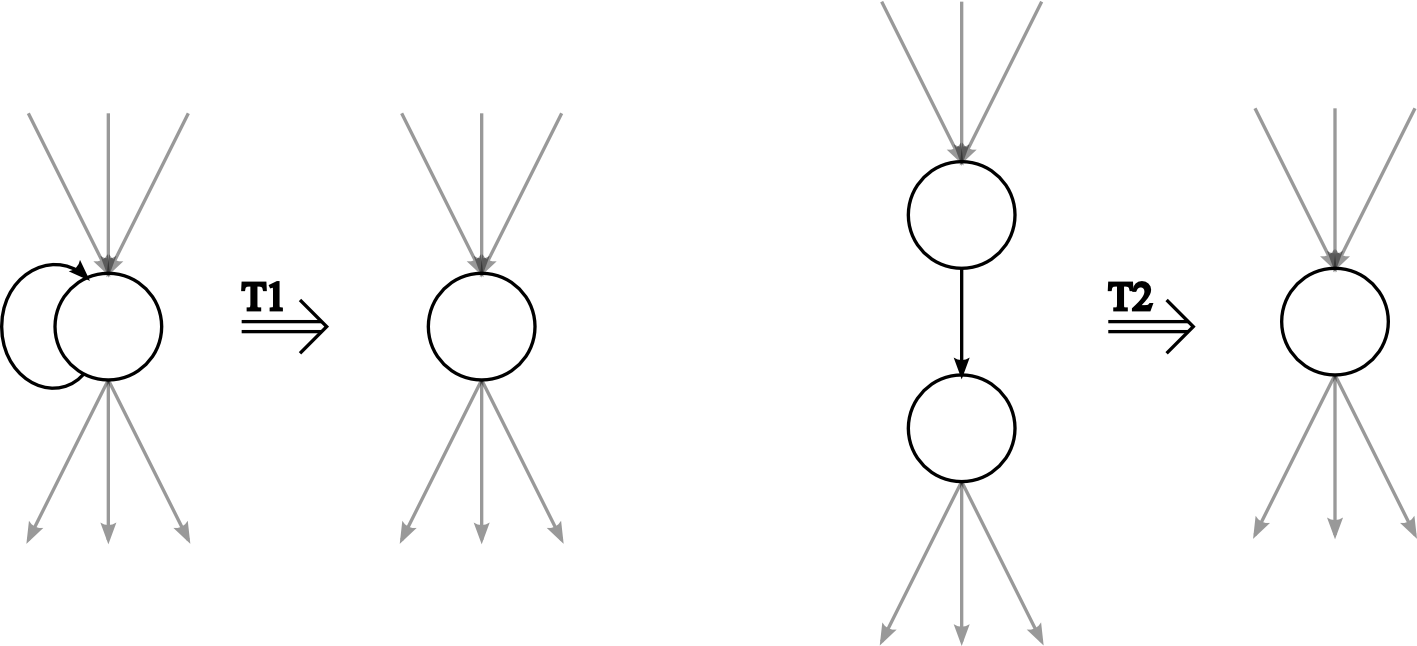
\includegraphics{figs/T1T2.png}}
\caption{\label{T1T2}T1 and T2 transformations}
\end{figure}

The T1 transformation removes self-loop.  If one of the successors
of a node is the node itself, then the node is a self-loop.
That is, the node `points' to itself.  The T1 transformation
replaces the node with a node without such link.
The number of preformed T1 transformations corresponds to the
number of loops in the program.

The T2 transformation merges two consecutive nodes together.
The only condition is the the second node has to have
only one predecessor which is the first node.
Preforming this transformation repeatedly basically reduces
any directed acyclic graph into a single node.

See figures \ref{IfThenElseReduction}, \ref{NestedLoops} and 
\ref{NestedLoops2} for examples how T1 and T2 transformations
can be used to reduce graphs.

\begin{figure}[p]
\centerline{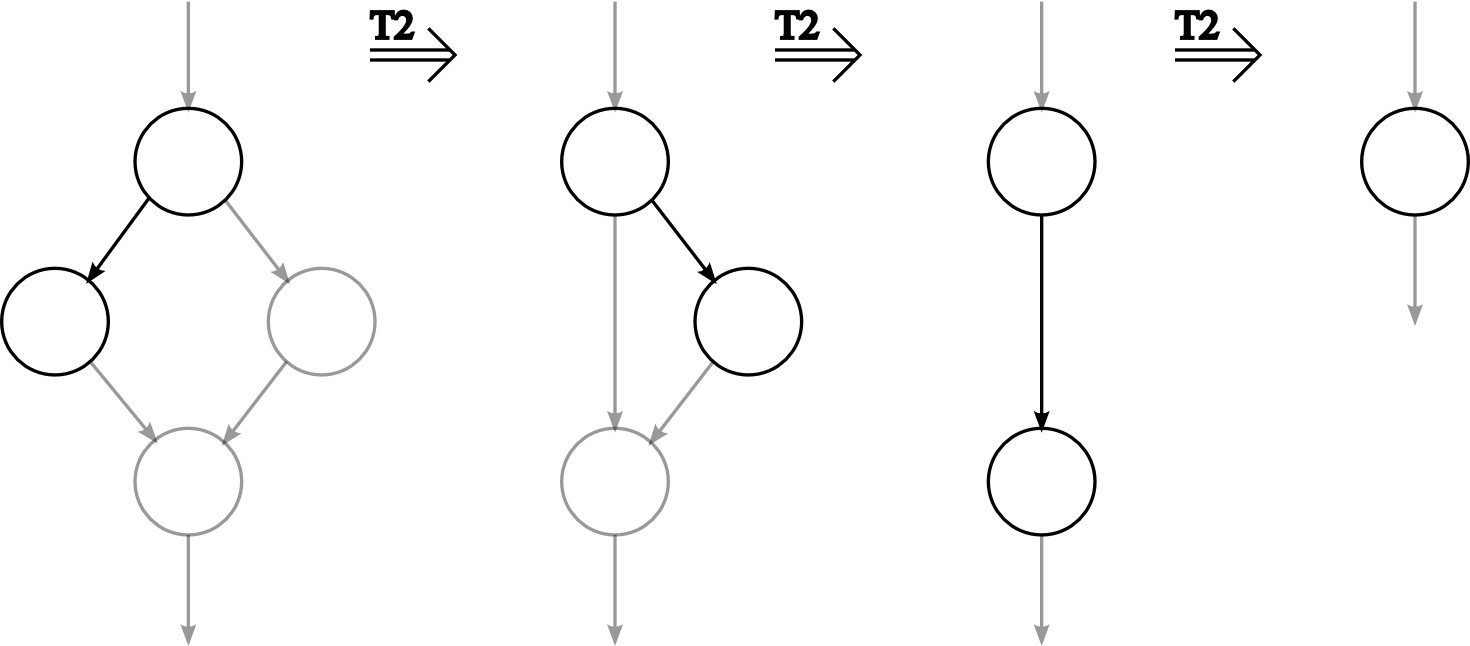
\includegraphics{figs/IfThenElseReduction.png}}
\caption{\label{IfThenElseReduction}Reduction of if-then-else statement}
\end{figure}

\begin{figure}[p]
\centerline{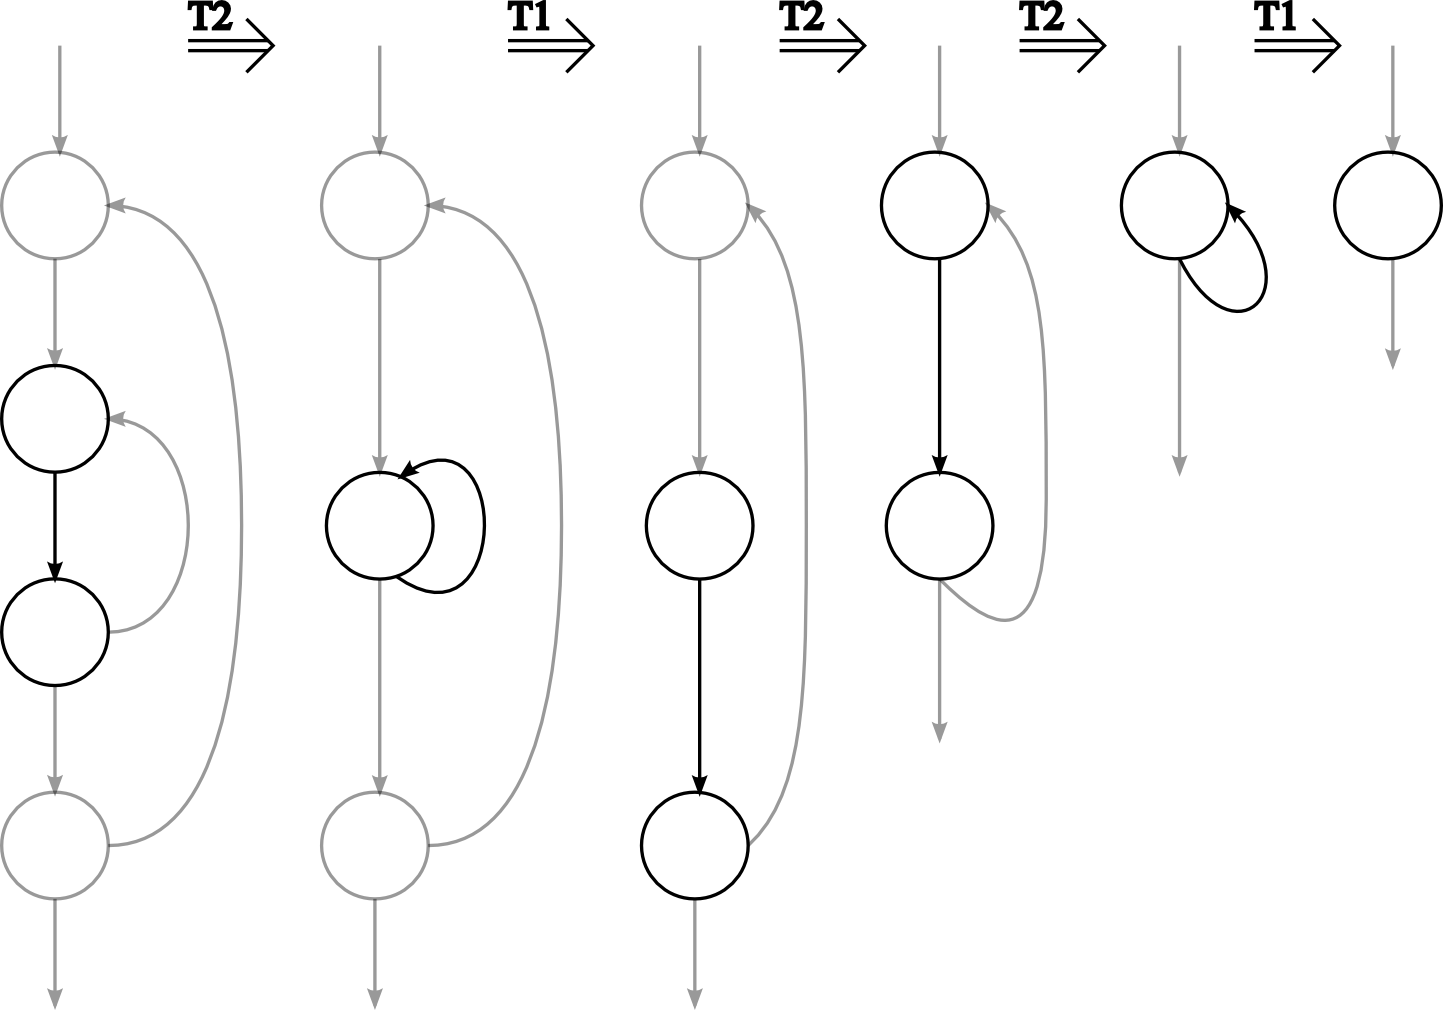
\includegraphics{figs/NestedLoops.png}}
\caption{\label{NestedLoops}Reduction of two nested loops}
\end{figure}

\begin{figure}[tbhp]
\centerline{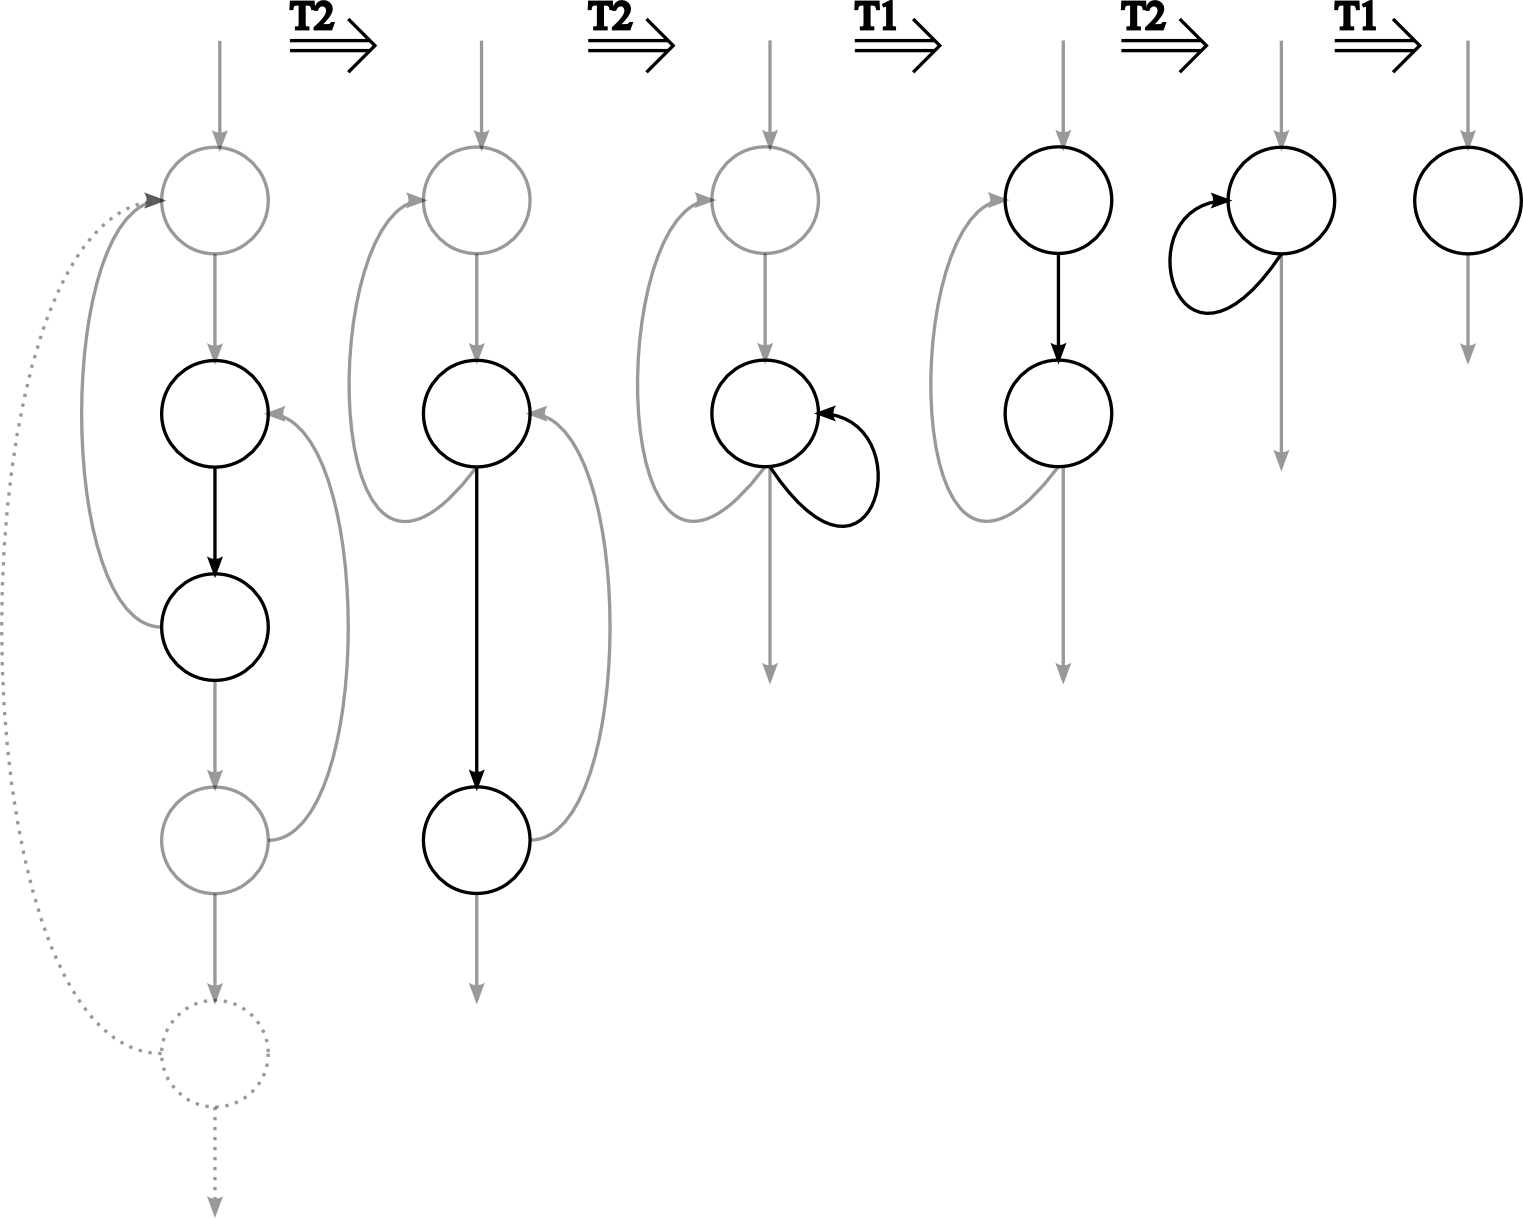
\includegraphics{figs/NestedLoops2.png}}
It is not not immediately obvious that these are, in fact,
two nested loops.  Fifth conceptual node has been added
to demonstrate why the loops can be considered nested.
\caption{\label{NestedLoops2}Reduction of two nested loops 2}
\end{figure}

The whole algorithm is guaranteed to terminate if and only
the graph is reducible.  However, it may produce different 
intermediate states depending on the order of the transformations.
For example, the number of T1 transformations used can vary.
This affects the number of apparent loops in the program.

Note that although reducible graphs are preferred,
irreducible graphs can be easily decompiled as well
using \verb|goto| statements.  Programs that were originally
written in C\# are most likely going to be reducible.

\subsection{Finding conditionals}
% Compound conditions

Any T1 transformation (self-loop reduction) produces a loop.
Similarly, T2 transformation or several T2 transformations
produce a directed acyclic sub-graph.  This sub-graph can
usually be represented as one or more conditional statements.

Any node in the control-flow graph that has two successors
is potentially a conditional -- that is, \verb|if-then-else|
statement.  The node itself determines which branch will
be taken, so the node is the condition.  We now need to
determine what is the `true' body and what is the `false'
body.  That is, we look for the blocks of code that will
be executed when the condition will or will not hold respectively.
This is done by considering reachability.  A code that is 
reachable only by following the `true' branch can be 
considered as the `true' body of the conditional.  
Similarly, code that is reachable only by following the
`false' branch is the `false' body of the conditional.
Finally, the code that is reachable from both branches is
not part of the conditional -- it is the code that follows
the whole \verb|if-then-else| statement.
See figure \ref{IfThenElseRechablility} for a diagram of this.

\begin{figure}[tbhp]
\centerline{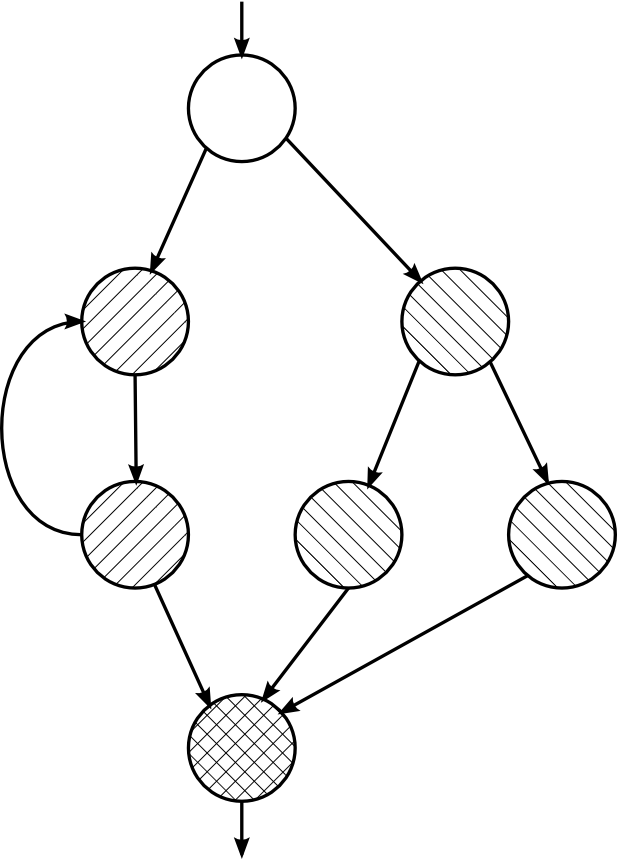
\includegraphics{figs/IfThenElseRechablility.png}}
\caption{\label{IfThenElseRechablility}Reachablity of nodes for a conditional}
\end{figure}

\subsection{Short-circuit boolean expressions}

Short-circuit boolean expressions are boolean expressions
which may not evaluate completely.

The semantics of normal boolean expression \verb|f() & g()| is
to evaluate both \verb|f()| and \verb|g()| and then return
the logical `and' of these.

The semantics of short-circuit boolean expression \verb|f() && g()|
is different.  The expression \verb|f()| is evaluated as before,
but \verb|g()| is evaluated only if \verb|f()| returned \emph{true}.
If \verb|f()| returned \emph{false} then the whole expression
will return \emph{false} anyway and so there no point in evaluating
\verb|g()|.

In general, conditionals depending on this short-circuit logic
cannot be expressed as normal conditionals without the use of \verb|goto|s
or code duplication.
Therefore it is desirable to find the short-circuit boolean expressions
in the control-flow graph.

The short-circuit boolean expressions will manifest themselves as
one of four patterns in the control-flow diagrams.
See figure \ref{shortcircuit}.

\begin{figure}[tbh]
\centerline{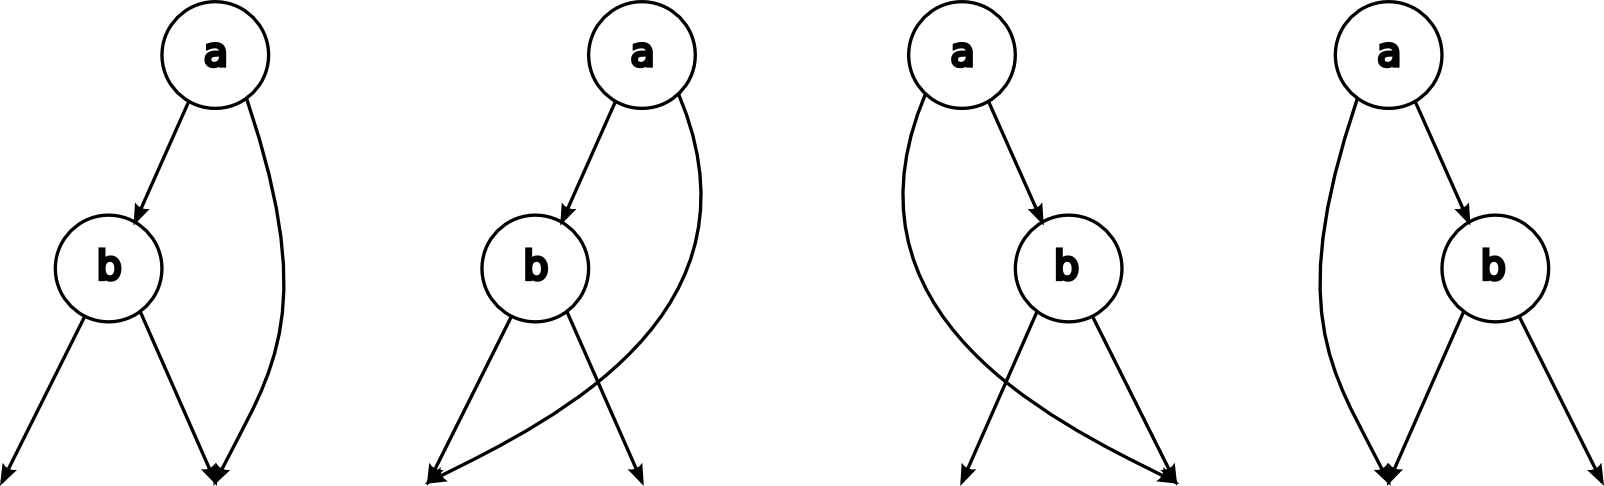
\includegraphics{figs/shortcircuit.png}}
\caption{\label{shortcircuit}Short-circuit control-flow graphs}
\end{figure}

These patterns can be easily searched for and replaced with a single node.

Nested expressions like \verb/(f() && g()) || (h() && i())/
will simplify well by applying the algorithm repeatedly.

\subsection{Basic blocks}
% Performance optimization only (from compilation)

Basic block is a block of code which is always executed as
a unit.  That is, no other code can jump in the middle of the 
block and there are no jumps from the middle of the block.

The implication of this is that as far as control-flow
analysis is concerned, the whole basic block can be 
considered as a single instruction.

This primary reason for implementing this is performance gain.


\section{Requirements Analysis}

The decompiler must successfully round-trip a quick-sort algorithm. 
That is, given an executable containing an implementation of
the quick-sort algorithm, the decompiler must produce
C\# source code that is both syntactically and semantically correct.
The produced source code must compile and work correctly
without any additional modifications to the source code.

To achieve this the Decompiler needs to handle at least the following:
\begin{itemize}
	\item Integers and integer arithmetic
	\item Create and be able to use integer arrays
	\item Branching must be successfully decompiled
	\item Several methods can be defined
	\item Methods can have arguments and return values
	\item Methods can be called recursively
	\item Integer command line arguments can be read and parsed
	\item Text can be outputted to the standard console output
\end{itemize}


\section{Development model}

The development is based on the spiral model.

The decompiler will internally consist of several consecutive code
representations.  The decompiled program will be gradually
transformed from one representation to other until it reaches
the last one and is outputted as source code.
This matches the spiral model well.  Successful implementation
of each code representation can be seen as one iteration in the
spiral model.

Furthermore, once a code representation is finished, it can
be improved by implementing an optimization which transforms it.
This can be seen as another iteration.


\section{Reference documentation}

The .NET executables will be decompiled into C\# source code.
It is therefore crucial to be intimately familiar with the language.
Evaluation semantics, operator precedence, associativity and other
aspects of the language can be found in the \emph{ECMA-334 Standard --
C\# Language Specification}.

In oder to decompile .NET executables, it is necessary to get
familiar with the .NET Runtime (i.e.\ the .NET Virtual Machine).
In particular, it is necessary to learn how the execution engine
works -- how does the stack behave, what limitations are imposed
on the code, what data types are used and so on.
Most importantly, it is necessary to get familiar with majority
of the bytecodes.
The primary reference for the .NET Runtime is the
\emph{ECMA-335 Standard -- Common Language Infrastructure (CLI)}.




%%%%%%%%%%%%%%%%%%%%%%%%%%%%%%%%%%%%%%%%%%%%%%%%%%%%%%%%%%%%%%%%%%%%%%%%%%%%%%%
% 25 Pages
\cleardoublepage
\chapter{Implementation}

\section{Development process}
% SVN
% GUI -- options; progressive optimizations
% Testing
% Refactoring

The whole project was developed in C\# on the \emph{Windows} platform.
SharpDevelop\footnote{Open-source integrated development environment
for the .NET framework.  I am actively participating in its development,
currently being one of the major developers.}
was used as the integrated development environment for writing of the code.

The source code and all files related to the project are stored on SVN%
\footnote{Subversion (SVN) is an open-source version control system.
It is very similar to CVS and aims to be its successor.}
server.  This has several advantages such as back-up of all data, 
documented project history (the commit messages) and the ability 
to revet back to any previous state.  The graphical user interface
for SVN also makes it possible to easily see and review all changes 
that were made since previous commit to the server.

The user interface of the decompiler is very simple.
It consists of a single window which is largely covered by a text area
containing the output of the decompilation process.
There are only a few controls in the top part of the window.
Several check boxes can be used to completely turn off or on 
optimization stages of the decompilation process.
Numerical text boxes can be used to specify the maximal number of
interactions for several transformations.  By gradually increasing
these it is possible to observe changes to the output step-by-step.
These options significantly aid in debugging and testing of 
the decompiler.

The source code generated by the decompiler is also stored on
the disk and committed to SVN together with all other files.
This is the primary method of regression testing.  The generated source code
is the primary output of the decompiler and thus any change 
in it may potentially signify a regression in the decompiler.
Before every commit the changes to this file were reviewed
to confirm that the new features did yield the expected 
results and that no regressions were introduced.


\section{Overview of representation structures}
% Stack-based bytecode
% Variable-based bytecode
% High-level blocks
% Abstract Syntax Tree

The decompiler uses the following four intermediate representations
of the program (sequentially in this order):
\begin{itemize}
\item Stack-based bytecode
\item Variable-based bytecode
\item High-level blocks
\item Abstract Syntax Tree
\end{itemize}
The code is translated from one representation to other and some
transformations/optimizations are done at each of these representations.

The representations are very briefly described in the following
four subsections and then they are covered again in more detail.

Trivial artificial examples are used to aid the explanation.
Note that the evaluation chapter shows the actual outputs
for the quick-sort implementation.

\subsection{Stack-based bytecode representation}
The stack-based bytecode is the original bytecode as read from the
assembly.  It is never modified.  However, it is analyzed and
annotated with the results of the analysis.  Most data-flow
analysis is performed at this stage.
This is an example of code in this representation:
\begin{verbatim}
ldstr "Hello, world!"
call System.Console::WriteLine
\end{verbatim}

\subsection{Variable-based bytecode representation}
The variable-based bytecode is the result of removing the
stack-based data-flow model.  Local variables are now used instead.
Even though the stack-based model is now completely removed,
we can still use the bytecodes to represent the program.
We just need to think about them in a slightly different way.
The bytecodes are in essence functions which take arguments
and return values.  For example, the \verb|add| bytecode
pops two values and pushes back the result and so it is now
a function which takes two arguments and returns the result.
The \verb|ldstr "Hello, world!"| bytecode used above is slightly
more complicated.  It does not pop anything from the stack,
but it still has the implicit argument \verb|"Hello, world!"|
which comes from the immediate operand of the bytecode.

Continuing with the example, the variable-based from would be:
\begin{verbatim}
temp1 = ldstr("Hello, world!");
call(System.Console::WriteLine, temp1);
\end{verbatim}
where the variable \verb|temp1| was used to remove the stack data-flow model.

Some transformations are performed at this stage, modifying the
code.  For example, the in-lining optimization would transform
the previous example to:
\begin{verbatim}
call(System.Console::WriteLine, ldstr("Hello, world!"));
\end{verbatim}
Note that expressions can be be nested as seen in the code above.

\subsection{High-level blocks representation}
The next data representation introduces high-level blocks.
In this representation, related parts of code can be grouped 
together into a block of code.
The block signifies some high-level structure and blocks can 
be nested (for example, conditional within a loop).
All control-flow analysis is performed at this stage.

The blocks can be visualized by a pair of curly braces:
\begin{verbatim}
{ // Block of type 'method body'
  IL_01: call(System.Console::WriteLine, ldstr("Hello, world"));
  { // Block of type 'loop'
    IL_02: call(System.Console::WriteLine, ldstr("!"));
    IL_03: br(IL_02) // Branch to IL_02
  }
}
\end{verbatim}
Initially there is only one block containing the whole method
body and as the high-level structures are found, new smaller
blocks are created.  At this stage the blocks have no function
other than grouping of code.

% Validity -- gotos
This data representation also allows code to be reordered
to better fit the ordinal high-level structure.

\subsection{Abstract Syntax Tree representation}

This is the final representation.  The abstract syntax tree (AST)
is a structured way of representing the produced source code.
For example, the expression \verb|(a + 1)| would be represented
as four objects -- parenthesis, binary operator, identifier and
constant.  The structure is a tree so the identifier and the constant
are children of the binary operator which is in turn child of the
parenthesis.

% The high-level structures are directly translated to nodes in the
% abstract syntax tree.  For example, loop will translate to 
% a node representing code \verb|for(;;) {}|.

% The bytecodes are translated to the abstract syntax tree on
% individual basis.  For example, the bytecode expression \verb|add(1, 2)| 
% is translated to \verb|1 + 2|.  The previously seen
% \verb|call(System.Console::WriteLine, ldstr("Hello, world"))|
% is translated to \verb|System.Console.WriteLine("Hello, world")|.

This initial abstract syntax tree will be quite verbose due to
constructs that ensure correctness of the produced source code.
There will be an especially high quantity of \verb|goto|s and
parentheses.  For example, a simple increment is initially
represented as \verb|((i) = (i) + (1));| where the parentheses
are used to ensure safety.
Transformations are done on the abstract syntax tree to simplify the code
in occasions where it is know to be safe.

Several further transformations are done to make the code more readable.
For example, renaming of local variables or use of common 
programming idioms.

\section{Stack-based bytecode representation}
  \label{Stack-based bytecode representation}

This is the first and simplest representation of the code.
It directly corresponds to the bytecode in the .NET executable.
It is the only representation which is not transformed in any way.

% Cecil
% Offset, Code, Operand
The bytecode is loaded from the .NET executable with the 
help of the Cecil library. 
Three fundamental pieces of information are loaded for each bytecode -- 
its offset from the start of the method, opcode
(name) and the immediate operand.  
The immediate operand is additional argument
present for some bytecodes -- for example, for the \verb|call| bytecode,
the operand specifies the method that should be called.

% Branch target, branches here
For bytecodes that can branch, the operand is the branch target.
Each bytecode stores a reference to the branch target (if any) and
each bytecode also stores a reference to all bytecodes that can branch to it.

\subsection{Stack analysis}

Once all bytecodes are loaded, the stack behavior of the program is analyzed.  
The precise state of the stack is determined for each bytecode.
The .NET Framework dictates that this must be possible for valid executables.
It is possible to determine the exact number of elements on the
stack and for each of these elements is possible to determine which bytecode
pushed it on the stack%
\footnote{In some control merge scenarios, there might be more 
bytecodes that can, depending on the execution path, push the value on the stack.}
and what the type of the element is.

% Stack before / after
% StackBehaviour -- difficult for methods
There are two stack states for each bytecode -- the first is the known
state \emph{before} the bytecode is executed and the second is the state
\emph{after} the bytecode is executed.  Knowing what the bytecode does,
the later state can be obviously derived from the former.  
This is usually easy -- for example, the \verb|add| bytecode pops 
two elements from the stack and pushes one back.  The pushed element
is obviously pushed by the \verb|add| bytecode 
and the element is of the same type as the two popped elements%
\footnote{The 'add' bytecode can only sum numbers of the same type.}.
The \verb|ldstr| bytecode just pushes one element of type \verb|string|.
The behaviour of the \verb|call| bytecode is slightly more complex 
because it depends on the method that it is invoking.  
Implementing these rules for all bytecodes is
tedious, but usually straightforward.

The whole stack analysis is performed by iterative algorithm.
The stack \emph{before} the very first bytecode is empty.
We can use this to find the stack state \emph{after} the first instruction.
The stack state \emph{after} the first bytecode is the 
initial stack state for other bytecode.
We can apply this principle again and again until all states are known.

% Branching -- 1) fall 2) branch 3) fall+branch    veryfy same
Branching dictates the propagation of the states between bytecodes.
For two simple consecutive bytecodes, the stack state \emph{after}
the first bytecode is same as the state \emph{before} the second.
Therefore we just copy the state.
If the bytecode is a branch then we need to copy
the stack state to the target of the branch as well.

Dead-code can never be executed and thus it does not have
any stack state associated with it.

At the bytecode level, the .NET Runtime handles boolean values
as integers.  For example, the bytecode \verb|ldc.i4 1| can
be interpreted equivalently as `push \verb|1|' and `push \verb|true|'.
Therefore three integer types are used -- 
`zero integer', `non-zero integer' and generic `integer' (of
unknown value).  Bytecode \verb|ldc.i4 1| therefore has type 
`non-zero integer'.

\section{Variable-based bytecode representation}
  \label{Variable-based bytecode representation}
% Removed stack-based model -- local variables, nesting

This is a next representation which differs from the stack-based
one by completely removing the stack-based data-flow model.
Data is passed between instructions using local variables
or using nested expressions.

Consider the following stack-based program which evaluates
$2 * 3 + 4 * 5$.
\begin{verbatim}
ldc.i4 2
ldc.i4 3
mul
ldc.i4 4
ldc.i4 5
mul
add
\end{verbatim}

The program is transformed to the variable-based form by
interpreting the bytecodes as functions which return values.
The result of every function call is stored in new temporary
variable so that the value can be referred to latter.

\begin{verbatim}
int temp1 = ldc.i4(2);
int temp2 = ldc.i4(3);
int temp3 = mul(temp1, temp2);
int temp4 = ldc.i4(4);
int temp5 = ldc.i4(5);
int temp6 = mul(temp4, temp5);
int temp7 = add(temp3, temp6);
\end{verbatim}

The stack analysis performed earlier is used to determine
what local variables should be used as arguments.
For example, the stack analysis tells us that the stack contains
precisely two elements just before the \verb|add| instruction.
It also tells us that these two elements have been pushed on the stack by the
\verb|mul| instructions (the third and sixth instruction respectively).
Therefore to access the results of the \verb|mul| instructions,
the \verb|add| instruction needs to use the temporary variables 
\verb|temp3| and \verb|temp6|.

\subsection{Representation}

Internally, each expression (`function call') consists of three 
main elements -- the opcode (e.g.\ \verb|ldc.i4|), the immediate operand
(e.g.\ \verb|1|) and the arguments (e.g.\ \verb|temp1|).
The argument can be either a reference to a local variable or 
other nested expression. In the case of
\begin{verbatim}
call(System.Console::WriteLine, ldstr("Hello, world"))
\end{verbatim}
\verb|call| is the opcode, 
\verb|System.Console::WriteLine| is the operand and
\verb|ldstr("Hello, world")| is the argument (nested expression).

Expressions like \verb|ldstr("Hello, world")| or \verb|ldc.i4|
do not have any arguments other then the immediate operand.

% stloc, ldloc
There are bytecodes for storing and referencing a local variables
(\verb|ldloc| and \verb|stloc| respectively).
Therefore no special data structures are needed to declare
and reference the local variables because we we can store 
program like
\begin{verbatim}
int temp1 = ldc.i4(2);
int temp2 = ldc.i4(3);
int temp3 = mul(temp1, temp2);
\end{verbatim}
only using bytecodes as
\begin{verbatim}
stloc(temp1, ldc.i4(2));
stloc(temp2, ldc.i4(3));
stloc(temp3, mul(ldloc(temp1), ldloc(temp2)));
\end{verbatim}

% Dup
Local variables \verb|temp1|, \verb|temp2| and \verb|temp3| 
are tagged as being `single static assignment and single read'.
This is a necessary property for the in-lining optimization.
All generated temporary variables satisfy this property
except for the ones storing the result of a \verb|dup| instruction 
which does not satisfy this property because it is read twice.

\subsection{In-lining of expressions}
     \label{In-lining of expressions}

The variable-based representation passes data between instructions
either using local variables or using expression nesting.
Expression nesting is the preferred more readable form.
The in-lining transformations simplifies the code by removing
some temporary variables and using expression nesting instead.

Consider the following code.
\begin{verbatim}
stloc(temp1, ldstr("Hello, world!"));
call(System.Console::WriteLine, ldloc(temp1));
\end{verbatim}
This code can be simplified into a single line by in-lining the
local variable \verb|temp1|:
(that is, the \verb|stloc| expression is nested within the
\verb|call| expression)
\begin{verbatim}
call(System.Console::WriteLine, ldstr("Hello, world!"));
\end{verbatim}

The algorithm is iterative.  Two consecutive lines are considered
and if the first line assigns to a local variable which is used
in the second line then the variable is in-lined.
This is repeated until no more optimizations can be done.

There are some safety concerns with this optimizations.
The optimization would break the program if the local variable
was read later in the program.
Therefore the optimization is done only for variables that have 
the property of being `single static assignment and single read'.

The second concern is change of execution order.
Consider the following pseudo-code:
\begin{verbatim}
temp1 = f();
add(g(), temp1);
\end{verbatim}
In-ling \verb|temp1| would change the order in which the
functions \verb|f| and \verb|g| are called and thus the 
optimization can not be performed.
On the other hand, the following code can be optimized:
\begin{verbatim}
temp1 = f();
add(1, temp1);
\end{verbatim}
The effect of the optimization will be that the expression
\verb|1| will be evaluated before \verb|f| rather then 
after it.  However, this does not change the semantics 
of the program because evaluation of \verb|1| does not have 
any side-effects and it will still evaluate to the same value.

More importantly, the same property holds for \verb|ldloc| (load local variable)
instruction.  It does not have any side-effects and it will 
evaluate to the same value even if evaluated before the
function \verb|f| (or any other expression being in-lined).
This is true because the function \verb|f|
(or any other expression being in-lined)
can not change the value of the local variable.  
% The only way to change a local 
% variable would be using the \verb|stloc| instruction.
% However, \verb|stloc| can not be part of the in-lined 
% expression because it does not return any value -
% it is a statement and as such can not be nested within an expression.

% The property holds for \verb|1|, \verb|ldloc| and it would hold
% for some other expressions as well, but due to the
% way the stack-based model was removed it is sufficient
% to consider only \verb|ldloc|.  This is by far the most common case.

To sum up, it is safe to in-line a local variable if it has
property `single static assignment and single read' and 
if the argument referencing it is preceded only 
by \verb|ldloc| instructions.

The following code would be optimized in two iterations:
\begin{verbatim}
stloc(temp1, ldc.i4(2));
stloc(temp2, ldc.i4(3));
stloc(temp3, mul(ldloc(temp1), ldloc(temp2)));
\end{verbatim}
First iteration (in-line \verb|temp2|):
\begin{verbatim}
stloc(temp1, ldc.i4(2));
stloc(temp3, mul(ldloc(temp1), ldc.i4(3)));
\end{verbatim}
Second iteration (in-line \verb|temp1|):
\begin{verbatim}
stloc(temp3, mul(ldc.i4(2), ldc.i4(3)));
\end{verbatim}


\subsection{In-lining of `dup' instruction}

The \verb|dup| instruction can not be in-lined because
it does not satisfy the `single static assignment and single read'
property.  This is because the data is referenced twice.
For example, in-lining the following code would cause 
the function \verb|f| to be called twice.
\begin{verbatim}
stloc(temp1, dup(f()));
add(temp1, temp1);
\end{verbatim}
However, there are circumstances where this would be acceptable.
If the expression within the \verb|dup| instruction is a 
constant then it is possible to in-line it without any harm.
The following code can be optimized:
\begin{verbatim}
stloc(temp1, dup(ldc.i4(2)));
add(temp1, temp1);
\end{verbatim}
Even more elaborate expressions like 
\verb|mul(ldc.i4(2), ldc.i4(3))| are still a constant.
The instruction \verb|ldarg.0| (load \verb|this|) is also
constant relative to the single invocation of method.



\section{High-level blocks representation}
  \label{High-level blocks representation}
% Links
% Link regeneration

So far the code is just a sequential list of statements.
The statements are in the exactly same order as found in the 
original executable and all control-flow is achieved 
only by the \verb|goto| statements.

The `high-level block' representation structure introduces
greater freedom to the code.  High-level structures are recovered 
and the code can be arbitrarily reordered.

The code is organized into blocks in this representation. 
A block can can contain executable code as well as other nested blocks.
Therefore this resembles a tree-like data structure.
The root block of the three represents the method and contains
all of its code.
A node in the three represents some high-level data structure
(loop, \verb|if| statement).  Nodes can also represent `meta'
high-level structures which are used during the optimizations.
For example, node can encapsulate a block of code that is known
to be acyclic (without loops).
Finally, all leaves in the tree are basic blocks.

\subsection{Safety}
This data representation allows the code to be restructured
and reordered.  Therefore care is needed to make sure that
the produced code is semantically correct.

% Validity -- arbitrary nodes
It would be possible to make sure that every transformation is 
valid.  However, there is even more robust solution --
give up at the start and allow arbitrary transformations.
The only constraint is that the code can be only moved.  It cannot
be duplicated and it cannot be deleted.  Deleting of code would
indeed cause problems.  Anything else is permitted.

When the code is generated, the correctness is ensured by
explicit \verb|label|s and \verb|goto|s placed in front
of and after every basic block respectively.  For example
consider the follow piece of code in which the order of
basic blocks was reversed and two unnecessary high-level 
nodes were added:

\begin{verbatim}
goto BasicBlock1; // Method prologue

for(;;) {
  BasicBlock2:
  Console.WriteLine("world");
  goto End;
}

if (true) {
  BasicBlock1:
  Console.WriteLine("Hello");
  goto BasicBlock2;
}

End:
\end{verbatim}

The inclusion of explicit \verb|label|s and \verb|goto|s
makes the high-level structures and the order of basic blocks
irrelevant and thus the produced source code will be correct.
Note that in the code above the lines \verb|for(;;) {| and 
\verb|if (true) {| will never be reached during execution.

In general, the transformations done on the code will be
more sane then in the example above and most of the
\verb|label|s and \verb|goto|s will be redundant.
In the following code all of the \verb|label|s and \verb|goto|s
can be removed:

\begin{verbatim}
goto BasicBlock1; // Method prologue

BasicBlock1:
Console.WriteLine("Hello");
goto BasicBlock2;

BasicBlock2:
Console.WriteLine("world");
goto End;

End:
\end{verbatim}

The removal of \verb|label|s and \verb|goto|s is done once
the Abstract Syntax Tree is created.

To sum up, finding and correctly identifying all high-level
structures will produce nice results, but failing to
do so will not cause any harm as far as correctness is concerned.


\subsection{Tree data structure}

The data structure to store the tree is very simple -- 
the tree consists of nodes where each node contains a link
to its parent and a list of children.  A child can be either
another node or a basic block (leaf).

The API of the tree structure is severely restricted.
Once the tree is created, it is only possible to add new empty 
nodes and to move basic blocks from one node to other.
This ensures that basic blocks can not be duplicated or
deleted which is the safety requirement as discussed in the
previous section.
All transformations are limited by this constraint.

Each node also provides events which are fired whenever
the child collection of the node is changed.

\subsection{Creating basic blocks}

The previous data representation stored the code as a sequence 
of statements.  Some of these statements will be always
executed sequentially without interference of branching.
In control-flow analysis we are primarily interested in
branching and therefore it is desirable to group such
sequential parts of code together to basic blocks.

Basic block is a block of code that is always guaranteed to
be executed together without any branching.  Basic blocks
can be easily found by determining which statements start
a basic block.  The very first statement in a method 
naturally starts the first basic block.  Branching transfers
control somewhere else so the statement immediately following
a branch is a start of a basic block.
Similarly, the target of a branch command is a start of
basic block.

Using these three simple rules the whole method body
is slit into a few basic blocks.

It is desirable to store control-flow links between basic blocks.  
These links are used for finding high-level structures.  
Each basic block has \emph{successors} and \emph{predecessors}.  
\emph{Successor} is an other basic block that may be executed
immediately after this one.
There can be up to two \emph{successors} -- the following basic 
block and the basic block being branched to.  Both of these
exist if the basic block ends with conditional branch.
% If the condition is false, the control falls though to the 
% following block and if the condition is true the branch is taken.
\emph{Predecessor} is just link in the opposite direction 
of the \emph{successor} link.  Note that the number of 
\emph{predecessors} is not limited -- several \verb|goto|s
can branch to the same location.


\subsection{Control-flow links between nodes}

The \emph{predecessor} and \emph{successor} links of basic
blocks reflect the control flow between basic blocks.
However, once basic blocks are `merged' by moving them
into a node, we might be interested in flow properties
of the whole node rather then just the individual basic blocks.
Consider two sibling nodes that represent two loops.
In other to put the nodes in correct order, we need to know
which one is \emph{successor} of the other.

Therefore the \emph{predecessor} and \emph{successor} links
apply to whole nodes as well.  Consider two sibling nodes $A$ and $B$.
Node $B$ is a \emph{successor} of node $A$ if there exists 
a basic block within node $A$ that branches to a basic block 
within node $B$.

The algorithm to calculate \emph{successors} of a node is
as flows:
\begin{itemize}
	\item Get a list of all basic blocks that are children of
	node $A$.  The node can contain other nested nodes so this part
	needs to be performed recursively.
	\item Get a list of all succeeding basic blocks of node $A$.
	This is the union of all successors for all basic blocks 
	within the node.
	\item However, we do not want succeeding basic blocks,
	we want a succeeding siblings of the node.  Therefore,
	for each succeeding basic block traverse the data structure
	up until a sibling node is reached.
\end{itemize}

The algorithm to calculate \emph{predecessors} of a node is similar.

The \emph{predecessor} and \emph{successor} links are used
extensively and it would be computationally expensive to 
recalculate them every time they are needed.  Therefore the
links and intermediate results of the calculation are cached.
The events of the tree structure are used to invalidate relevant
caches.

\subsection{Finding loops}
     \label{Finding loops}

The loops are found by using the T1-T2 transformations which where
discussed in the preparation chapter.

There are two node types that directly correspond to the results
of these two transformations.  Preforming a T1 transformation
produces a node of type \emph{Loop} and performing a T2 transformation
produces a node of type \emph{AcyclicGraph}.

The algorithm works by considering all the nodes and basic blocks
in the tree individually and evaluating the conditions required for the
transformations.
If transformation can be performed for a given node, it is immediately
preformed and the algorithm is restarted on the new transformed graph.
The condition for the T1 transformation (\emph{Loop}) is that the node
must a be self-loop.  The condition for the T2 transformation
(\emph{AcyclicGraph}) is that the node must have only one predecessor.

By construction each \emph{AcyclicGraph} node contains exactly
two nodes.  For example, five sequential statements would be
represented as four nested \emph{AcyclicGraph} nodes.
This makes the tree more complex and more difficult to analyse.
The acyclic property is only required for loop finding and is not
needed for anything else later on.  Therefore once loops are found,
the \emph{AcyclicGraph} nodes are flattened (the children of the node
are moved to its parent and the node is removed).

Note that the created loops are trivial -- the \emph{Loop} node
represents an infinite loop without initializer, condition or
iterator.  The specifics of the loop are not represented
in this tree data structure.  However, they are eventually
recovered in the abstract syntax tree phase of the decompiler.

\subsection{Finding conditionals}
     \label{Finding conditionals}
% Reachable sets

In order to recover conditional statements three new node types
are introduced: \emph{Condition}, \emph{Block} and \emph{IfStatement}.
\emph{Condition} represents a piece of code that is guaranteed to 
branch into one of two locations.  \emph{Block} has no special
semantics and merely groups several nodes into one.
\emph{IfStatement} represents the whole conditional including
the condition and two bodies.

The \emph{IfStatement} node is still a genuine node in the tree
data structure.  However, subtyping is used to restrict its children.
The \emph{IfStatement} node must have precisely three children
of types \emph{Condition}, \emph{Block} and \emph{Block} representing
the condition, `true' body and `false' body respectively.
This defines the semantics of the \emph{IfStatement} node.

The algorithm starts by encapsulating all two-successors basic blocks 
with \emph{Condition} node.  Two-successor basic blocks are conditional
branches and thus they are conditions of \verb|if| statements.
Note that the bytecode \verb|br| branches unconditionally and thus
is it not a condition of an \verb|if| statement (basic blocks ending
with \verb|br| have only one successor).

The iterative part of the algorithm is to look for free-standing
\emph{Condition} nodes and encapsulate them with \emph{IfStatement} nodes.
This involves finding the `true' and `false' bodies for the if statements.

The `true' and `false' bodies of an \verb|if| statement are found by
considering reachability as discussed in the preparation chapter.
Nodes reachable only by following the `true' branch define the `true'
body of the \verb|if| statement.  Similarly for the `false' body.
The rest of the nodes is the set reachable from both and it is not
part of the \verb|if| statement -- it is the code following the 
\verb|if| statement.  Note that these three set are disjoint.

The reachable nodes nodes are found by iterative algorithm in 
which successors are added to a collection until the collection
does not change anymore.
Nodes that are reachable \emph{only} from the `true' branch are 
obtained by taking the set reachable from `true' branch and removing
nodes reachable from the `false' branch.

Consider the special case where there are no nodes reachable from both
the `true' and `false' branches.  In this case, there is no code 
following the \verb|if| statement.  Such code might look like this:
\begin{verbatim}
if (condition) {
  return null;
} else {
  return result;
}
\end{verbatim}

In this special case the `false' body is moved outside the \verb|if|
statement producing more compact code:
\begin{verbatim}
if (condtion) {
  return null;
}
return result;
\end{verbatim}


\subsection{Short-circuit conditionals}
% Short-circuit

Consider condition like \verb|a & b| (\verb|a| and \verb|b|).
This or even more complex expressions compile into a code without
any branches.  Therefore the expression will be contained within
a single basic block and thus the approach described so far 
would work well.

Conditions like \verb|a && b| are more difficult to handle 
(\verb|a| and \verb|b|, but evaluate \verb|b| only if \verb|a|
is true).  These short-circuit conditionals introduce additional
branching and thus they are more difficult to decompile.

% The short-circuit conditionals will manifest themselves as 
% one of four flow graphs.  See figure \ref{impl_shortcircuit}
% (repeated from the preparation chapter).

% Implementation
% \begin{figure}[tbh]
% \centerline{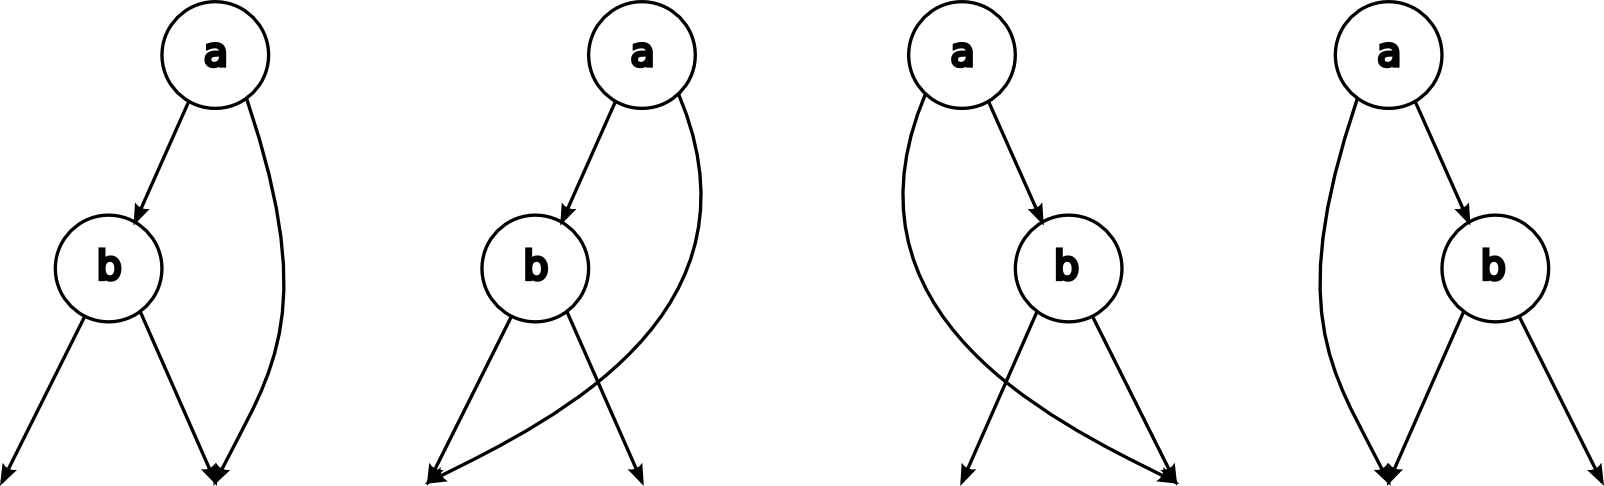
\includegraphics{figs/shortcircuit.png}}
% \caption{\label{impl_shortcircuit}Short-circuit control-flow graphs}
% \end{figure}

The expression \verb|a| is always evaluated first.
The flow graph is characterized by two things -- in which case the 
expression \verb|b| is evaluated and which path is taken if the
expression \verb|b| is not evaluated.

The \emph{Condtition} node was previously defined as a piece of 
code that is guaranteed to branch into one of two locations.
This still holds for the flow graphs above.  If two nodes 
that evaluate \verb|a| and \verb|b| are considered together,
they still define a proper condition for an \verb|if| statement.
We define a new node type \emph{ShortCircuitCondition}
which is a special case of \emph{Condition}.  
This node has exactly two children (expressions \verb|a| and 
\verb|b|) and a meta-data field which specifies which one of 
the four short-circuit patters it represents.  This is for
convenience so that the pattern matching does not have to be
done again in the future.

The whole program is repeatedly searched and if one of the four patters 
is found, the two nodes are merged into a \emph{ShortCircuitCondition} node.
This new node represents the combined expression (e.g.\ \verb|a && b|).
Since it is a single node is eligible to fit into the pattern
again and thus nested short-circuit expressions will be also
found (e.g.\ \verb/(a && b) || (c && d)/).

Note that this is an extension to the previous algorithm rather
then a new one.  It needs to be preformed just before 
\emph{Condition} nodes are encapsulated in \emph{IfStatement} nodes.


\section{Abstract Syntax Tree representation}
  \label{Abstract Syntax Tree representation}

Abstract syntax tree (AST) is the last representation of the program.
It very closely corresponds to the final textual output.

\subsection{Data structure}

External library is used to hold the abstract syntax tree.

Initially the \emph{CodeDom} library that ships with the
\emph{.NET Framework} was used, but it was soon abandoned due
to lack of support for many crucial C\# features.

It was replaced with \emph{NRefactory} which is an open-source 
library used in SharpDevelop for parsing and representation of 
C\# and VB.NET files.
It focuses exclusively on these two languages and
thus provides excellent support for them.

NRefactory allows perfect control over the generated code.
Parsing arbitrary C\# file and then generating it again
will almost exactly reproduce the original text.  Whitespace
would be reformated but anything else is explicitly represented
in NRefactory's abstract syntax tree.
For example,  \verb|(a + b)| and \verb|a + b| have 
different representations and so do \verb|if (a) return;| and 
\verb|if (a) { return; }|.

The decompiler aims to generate not only correct code, but also as
readable code as possible.  Therefore this precise control is desirable.


\subsection{Generating skeleton}

The first task is to generate code skeleton that is
equivalent to the one in the executable.
The \emph{Cecil} library helps with reading of the executable
meta-data and thus it is not necessary to work directly with
the binary format of the executable.

The following four object types can be found in .NET executables:
classes, structures, interfaces and enumerations.
For the purpose of logical organization these can be nested 
within namespaces and, in some cases, nested within each other.
Classes can be inherited and may implement one or more interfaces.
Depending on the type, the objects can contain fields,
properties, events and methods.
Specific set of modifies can be applied to almost everything.

Handling all these cases is tedious, but usually straightforward.

\subsection{Generating method bodies}
     \label{Generating method bodies}

Once the skeleton is created, high-level blocks and the bytecode
expressions contained within them are translated to 
abstract syntax tree.  For example, the \emph{Loop} node is translated 
to a \emph{ForStatement} in the AST and the bytecode expression \verb|add|
is translated to \emph{BinaryOperatorExpression} in the AST.

In terms of lines of code, this is by far the largest part of the
decompiler.  The reason for this is that there are many bytecodes
and every bytecode needs to have its own specific translation code.

Conceptually\footnote{In reality there are more functions 
that are loosely coupled.},
the translation code consists of three main functions:
\emph{TranslateMethodBody}, \emph{TranslateHighLevelNode} and
\emph{TranslateBytecodeExpression}.
All of these return complete abstract syntax tree for the given input.

\emph{TranslateMethodBody} is the simples function which encapsulates
the whole algorithm.  It takes tree of high-level blocks as input and 
produces the complete abstract syntax tree of the method.
Internally, it calls \emph{TranslateHighLevelNode} for each top-level
node and then merely concatenates the results.

\emph{TranslateHighLevelNode} translates one particular high-level 
node into abstract syntax tree.  There are several types of high-level
nodes and each of them needs to considered individually.
If the high-level node has child nodes then this function is
called recursively.  Some comments about particular node types:
The \emph{BasicBlock} node needs to be preceded by explicit label
and succeeded by explicit \verb|goto| in order to ensure safety.
The \emph{Loop} node is easy to handle since it is just an infinite loop.
The \emph{IfStatement} node is most difficult to handle since it
needs to handle creation of the condition for the \verb|if| statement.
Remember, that the condition can include short-circuit booleans and
that these can be arbitrarily nested.

\emph{TranslateBytecodeExpression} is the lowest level function.
It translates the individual bytecode expressions.
Note that bytecode expression may have other bytecode expressions
as arguments and therefore this function is often called recursively.
Getting abstract syntax tree for all arguments is in fact the
first thing that is done.  After that these arguments are combined in
a way that is appropriate for the given bytecode and operand.
This logic is completely different for each bytecode.  
Simple example is the \verb|add| bytecode --  
in this case the arguments end up being children of 
\emph{BinaryOperatorExpression} (which is an AST node).
At this point we have the abstract syntax tree representing the 
bytecode expression. 
The expression is further encapsulated by parenthesis for safety
and the type of the expression is recoded in the AST meta-data.

Unsupported bytecodes are handled gracefully and are represented as
function calls.  For example if the \verb|add| bytecode would
not be implemented, it would be outputed as \verb|IL__add(1, 2)|
rather then \verb|1 + 2|.

Recoding the type of AST is useful so that it can be converted
depending on a context.  If AST of type \verb|IntegerOne| is
used in context where \verb|bool| is expected, the AST can
be simply replaced by \verb|true|.

Here is a list of bytecodes whose translation into abstract syntax
tree has been implemented
(star is used to represent several bytecodes with similar names):

Arithmetic: \texttt{add* div* mul* rem* sub* and xor shl shr* neg not} \\
Arrays: \texttt{newarr ldlen ldelem.* stelem.*} \\
Branching: \texttt{br brfalse brtrue beq bge* bgt* ble* blt* bne.un} \\
Comparison: \texttt{ceq cgt* clt*} \\
Conversions: \texttt{conv.*.*} \\
Object-oriented: \texttt{newobj castclass call callvirt} \\
Constants: \texttt{ldnull ldc.* ldstr ldtoken} \\
Data access: \texttt{ldarg ldfld stfld ldsfld stsfld ldloc stloc} \\
Miscellaneous: \texttt{nop dup ret}

The complexity of implementing a translation for a bytecode varies
between a single line (\verb|nop|) to over a page of code (\verb|callvirt|).


\subsection{Optimizations}

The produced abstract syntax tree represents a fully functional program.
That is, it can be pretty printed and the generated source code would 
compile and work without problems.  
However, the produced source code is still quite verbose and
therefore several optimizations are done to simplify it or make it `nicer'.

The optimizations are implemented by using the visitor pattern
provided by the NRefactory library.  For each optimization
a new class is created which inherits from the \emph{AstVisitor}
class.  Instance of this class is created and it is applied to 
the root of the abstract syntax tree.
As a result of this, NRefactory will traverse the whole abstract
syntax tree and notify the visitor (the optimization) about
every element it encounters.  For example, whenever a \verb|goto|
statement is encountered, the method \verb|VisitGotoStatement|
will be invoked on the visitor.  If the optimization wants to
act upon this, it has to override the \verb|VisitGotoStatement| method.
The abstract syntax tree can be modified during the traversal.
For example, when the \verb|goto| statement is encountered,
the visitor (the optimization) can modify it, replace it or simply
remove it.

\subsubsection{Removal of dead labels}
        \label{Removal of dead labels}

This is not the first optimization to be executed, but it is the 
simplest one and therefore it is explained first.

The purpose of this optimization is to remove dead labels.
That is, to remove all labels that are not referenced by one
or more \verb|goto| statements.

The optimization uses two visitors.  The first visitor overrides
the \verb|VisitGotoStatement| method and is thus notified about
all \verb|goto| statements in the method.  The body of the overridden
\verb|VisitGotoStatement| method records the name of the label
being targeted and puts in into an `alive' list.

The second visitor overrides the \verb|VisitLabelStatement|
method and is thus notified about all labels.  If the label
is not in the `alive' list, it is removed.

Note that all optimizations are done on per-method basis
and therefore we do not have to worry about name clashes
of labels from different methods.


\subsubsection{Removal of negations}
        \label{Removal of negations}

In some cases negations can be removed by using the rules of
logic.  Negations are represented as \emph{UnaryOperatorExpression}
in the abstract syntax tree.

When a negation is encountered, it is matched against the following 
patterns and simplified if possible.

\verb|!((x)) = !(x)| \\
\verb|!!(x) = (x)| \\
\verb|!(a > b) = (a <= b)| \\
\verb|!(a >= b) = (a < b)| \\
\verb|!(a < b) = (a >= b)| \\
\verb|!(a <= b) = (a > b)| \\
\verb|!(a == b) = (a != b)| \\
\verb|!(a != b) = (a == b)| \\
\verb:!(a & b) = (!(a) | !(b)): \\
\verb:!(a && b) = (!(a) || !(b)): \\
\verb:!(a | b) = (!(a) & !(b)): \\ 
\verb:!(a || b) = (!(a) && !(b)): \\

\subsubsection{Removal of parenthesis}
        \label{Removal of parenthesis}
% C precedence and associativity

To ensures safety, the abstract syntax tree will contain extensive
amount of parenthesis.  Even simple increment would be expressed
as \verb|((i) = ((i) + (1)))|.

This optimization removes parenthesis where it is known to be safe.

Parenthesis can be removed from primitive values (\verb|(1)|),
identifiers (\verb|(i)|) and already parenthesized expressions 
(\verb|((...))|).

Several parenthesis can also be removed due to the unambiguous
context they are in.  This includes cases like
\verb|return (...);|, \verb|array[(...)]|, \verb|if((...))|, 
\verb|(...);| and several others.

The rest of the cases is governed by the C\# precedence
and associativity rules.  There are 15 precedence groups in
C\# and expressions within the same group are left-associative%
\footnote{Only assignment and conditional operator (?:)
are right associative, but these are never generated in nested
form by the decompiler.}.

The optimization implements a function \verb|GetPrecedence| that
returns the precedence for the given expression as an integer.

Majority of expressions are binary expressions.  When a binary
expression is encountered, precedence is calculated for it
and both of its operands.
For example consider \verb|(a + b) - (c * d)|. 
The precedence of the main binary expression is 12 and the 
precedences of the operands are 12 and 13 respectively.
Since the right operand has higher precedence then the binary 
expression itself, its parenthesis can be removed.
The left operand has the same precedence.  However, in this special 
case (left operand, same precedence), parenthesis can be removed
as well due to left-associativity of C\#.

Similar, but simpler, logic applies to unary expressions.

\subsubsection{Removal of `goto' statements}
        \label{Removal of `goto' statements}
% Goto X; labe X: ;
% Replacing with break/continue

This is the most complex optimization performed on the
abstract syntax tree.  Its purpose is the remove or replace
\verb|goto| statements.

In the following case it is obvious that the \verb|goto| can be removed:
\begin{verbatim}
// Code
goto Label;
Label:
// Code
\end{verbatim}

However, in general, more complex scenarios can occur.
It is not immediately obvious that the \verb|goto| statement
can be removed in the following code:

\begin{verbatim}
if (condition1) {
  if (condition2) {
    // Code
    goto Label;
  } else {
    // Code
  }
}
for(;;) {
  for(;;) {
    Label:
    // Code
  }
}
\end{verbatim}

This optimization is based on simulation of execution under
various conditions.
There are three important questions that the simulation answers: \\
What would happen if the \verb|goto| was replaced by no-op (i.e.\ removed)? \\
What would happen if the \verb|goto| was replaced by \verb|break|? \\
What would happen if the \verb|goto| was replaced by \verb|continue|?

In the first case, the \verb|goto| is replaced by
no-op and the simulator is started at that location.
The simulation will traverse the AST tree structure until
it finds the next executable line of code or an label.
If the reached location is the same as the one that would be reached
by following the original \verb|goto| then the original \verb|goto|
can be removed.

Similar simulation runs are performed by replacing the
\verb|goto| by \verb|break| and \verb|continue|.



After this optimization is done, it is desirable to remove the dead labels.

\subsubsection{Simplifying loops}
        \label{Simplifying loops}

The \verb|for| loop statement has the following form in C\#:
\begin{verbatim}
for(initializer; condition; iterator) { body };
\end{verbatim}

The semantics of the \verb|for| loop statement is:
\begin{verbatim}
initializer;
for(;;) {
  if (!condition) break;
  body;
  iterator;
}
\end{verbatim}

So far the decompiler generated only infinite loops in form
\verb|for(;;)|.  Now it is time to make the loops more interesting.
This optimization does pattern matching on the code and tries
to identify the initializer, condition or iterator.

If the loop is preceded by something like \verb|int i = 0;| then it is most
likely the initializer of the loop and it will be pushed into
the \verb|for| statement producing \verb|for(int i = 0;;)|.
If it is not really the initializer, it does not matter -- 
semantics is same.

If the first line of the body is \verb|if (not_condition) break;|,
it is assumed to be the condition for the loop and it is pushed
in to produce \verb|for(;!not_condition;)|.

If the last line of the body is \verb|i = ...| or \verb|i++|,
it is assumed to be the iterator.

Consider the following code:
\begin{verbatim}
int i = 0;
for(;;) {
  if (i >= 10) break;
  // body
  i++;
}
\end{verbatim}

Performing this optimization will simplify the code to:
\begin{verbatim}
for(int i = 0; !(i >= 10); i++) {
  // body
}
\end{verbatim}

This is then further simplified by the `removal of negation'
optimization to:

\begin{verbatim}
for(int i = 0; i < 10; i++) {
  // body
}
\end{verbatim}


\subsubsection{Further optimizations}
        \label{Further optimizations}

Several further optimizations are done which are briefly
discussed here.

% Rename variables -- i, j,k ... 
Integer local variables are renamed from the more generic names
like \verb|V_0| to \verb|i|, \verb|j|, \verb|k|, and so on.
Boolean local variables are renamed to \verb|flag1|, \verb|flag2|
and so on.

% Type names
C\# aliases for types are used.  For example, \verb|System.Int32|
is replaced with \verb|int|.  C\# \verb|using| (\verb|import| in
java) is used to simplify \verb|System.Console| to just \verb|Console|.
Types in scope of same namespace also do not have to be
fully qualified.

% Remove `this' reference
Explicit \verb|this.field| is simplified to just \verb|field|.

% Idioms -- i++
The increments in form \verb|i = i + 1| are simplified to \verb|i++|.
The increments in form \verb|i = i + 2| are simplified to \verb|i += 2|.
Analogous forms hold for decrements.

% Idioms -- string concat, i++
String concatenation \verb|String.Concat("Hello", "world")|
can be expressed in C\# just as \verb|"Hello" + "world"|.

Sometimes `false' body of an \verb|if| statement can end up being
empty and can be harmlessly removed.

Some control-flow commands are sometimes redundant since the
implicit behavior is equivalent.  For example, \verb|return;|
at the end of method is redundant and \verb|continue;| at
the end of loop is redundant.


\subsection{Pretty Printing}

Pretty printing%
\footnote{Pretty printing is the act of converting abstract
syntax tree into a textual form.}
is provided as part of the NRefactory library and therefore does not
need to be implemented as part of the decompiler.
The NRefactory provides provides several options that control
the format of the produced source code (for example whether an opening 
curly brace is placed on the same line as \verb|if| statement or on
the following line).

NRefactory is capable to output the code both in C\# and in VB.NET.


%%%%%%%%%%%%%%%%%%%%%%%%%%%%%%%%%%%%%%%%%%%%%%%%%%%%%%%%%%%%%%%%%%%%%%%%%%%%%%%
% 10 Pages
\cleardoublepage
\chapter{Evaluation}

\newcommand{\impref}[1]{See section \emph{\ref{#1} #1} on page \pageref{#1} for reference.}

\section{Success Criteria}

The principal criterion was that the quick-sort algorithm must successfully
decompile.  This goal was achieved.
The decompiled source code is, in fact, almost identical to the original.
This is demonstrated at the end of the following section.

\section{Evolution of quick-sort}

This section demonstrates how the quick-sort algorithm is decompiled.

Four different representations are used during the decompilation process.
The output of each of these representations is shown.

Unless otherwise specified the shown pieces of code are 
verbatim outputs of the decompiler.

\subsection{Original source code}

To save space we will initially consider only the \verb|Main| method of
the quick-sort algorithm.  It parses textual arguments,
performs the quick-sort and then prints the result.

\begin{verbatim}
public static void Main(string[] args)
{
  int[] intArray = new int[args.Length];
  for (int i = 0; i < intArray.Length; i++) {
    intArray[i] = int.Parse(args[i]);
  }
  QuickSort(intArray, 0, intArray.Length - 1);
  for (int i = 0; i < intArray.Length; i++) {
    System.Console.Write(intArray[i].ToString() + " ");
  }
}
\end{verbatim}

This code is compiled with all optimizations turn on and its
binary form is considered is the following sections.

\subsection{Stack-based bytecode representation}
    \impref{Stack-based bytecode representation}

This is a snippet of the bytecode as loaded from the executable.  
This part represents the line \verb|intArray[i] = int.Parse(args[i]);|.
\verb|V_0| is \verb|intArray| and \verb|V_1| is \verb|i|.

Comments denote the stack behaviour of the bytecodes.

The (manually) stared bytecodes represent just the part
\verb|int.Parse(args[i]);|.

\begin{verbatim}
IL_0F: ldloc V_0          # Pop0->Push1   
IL_10: ldloc V_1          # Pop0->Push1   
IL_11: ldarg args      *  # Pop0->Push1   
IL_12: ldloc V_1       *  # Pop0->Push1   
IL_13: ldelem.ref      *  # Popref_popi->Pushref   
IL_14: call Parse()    *  # Varpop->Varpush Flow=Call  
IL_19: stelem.i4          # Popref_popi_popi->Push0   
\end{verbatim}

The used bytecodes are \verb|ldloc| (load local variable),
\verb|ldarg| (load argument), \verb|ldelem| (get array element),
\verb|call| (call method) and \verb|stelem| (set array element).

Here is the same snippet again after the stack analysis
has been performed.

\begin{verbatim}
// Stack: {}
IL_0F: ldloc V_0              # Pop0->Push1  
// Stack: {IL_0F}
IL_10: ldloc V_1              # Pop0->Push1  
// Stack: {IL_0F, IL_10}
IL_11: ldarg args             # Pop0->Push1  
// Stack: {IL_0F, IL_10, IL_11}
IL_12: ldloc V_1              # Pop0->Push1  
// Stack: {IL_0F, IL_10, IL_11, IL_12}
IL_13: ldelem.ref             # Popref_popi->Pushref  
// Stack: {IL_0F, IL_10, IL_13}
IL_14: call Parse()           # Varpop->Varpush Flow=Call 
// Stack: {IL_0F, IL_10, IL_14}
IL_19: stelem.i4              # Popref_popi_popi->Push0  
// Stack: {}
\end{verbatim}

For example, we can see that bytecode \verb|IL_13: ldelem.ref| pops 
the last two elements from the stack -- \verb|{IL_11, IL_12}|.
These will hold the values \verb|args| and \verb|V_1| respectively.

The bytecode \verb|IL_19: stelem.i4| pops three values.

\subsection{Variable-based bytecode representation}
    \impref{Variable-based bytecode representation}

This is the same snippet after the stack-based data-flow
is replaced with variable-based one:
(code manually simplified for clarity)

\begin{verbatim}
expr0D = ldloc(V_0);
expr0E = ldloc(i);
expr0F = ldarg(args);
expr10 = ldloc(i);
expr11 = ldelem.ref(expr0F, expr10);
expr12 = call(Parse(), expr11);
stelem.i4(expr0D, expr0E, expr12);
\end{verbatim}

Here is the actual unedited output:

\begin{verbatim}
stloc(expr0D, ldloc(V_0));
stloc(expr0E, ldloc(i));
stloc(expr0F, ldarg(args));
stloc(expr10, ldloc(i));
stloc(expr11, ldelem.ref(ldloc(expr0F), ldloc(expr10)));
stloc(expr12, call(Parse(), ldloc(expr11)));
stelem.i4(ldloc(expr0D), ldloc(expr0E), ldloc(expr12));
\end{verbatim}

\subsubsection{In-lining of expressions}
       \impref{In-lining of expressions}

Here is the same snippet after two in-lining optimizations.
(this is actual output -- the GUI of the decompiler allows performing
of optimizations step-by-step)

\begin{verbatim}
stloc(expr0D, ldloc(V_0));
stloc(expr0E, ldloc(i));
stloc(expr11, ldelem.ref(ldarg(args), ldloc(i)));
stloc(expr12, call(Parse(), ldloc(expr11)));
stelem.i4(ldloc(expr0D), ldloc(expr0E), ldloc(expr12));
\end{verbatim}

All posible in-lines are performed:

\begin{verbatim}
stelem.i4(ldloc(V_0), ldloc(i),
          call(Parse(), ldelem.ref(ldarg(args), ldloc(i))));
\end{verbatim}


\subsection{Abstract Syntax Tree representation (part 1)}
    \impref{Abstract Syntax Tree representation}

Let us omit the optimization of high-level structures
for this moment and skip directly to the Abstract Syntax Tree.

After transforming a snippet of code to variable-based bytecode
and then performing the in-lining optimization we have obtained

\begin{verbatim}
stelem.i4(ldloc(V_0), ldloc(i),
          call(Parse(), ldelem.ref(ldarg(args), ldloc(i))));
\end{verbatim}

Let us see the same result for larger part of the method:

\begin{verbatim}
BasicBlock_1: stloc(V_0, newarr(System.Int32,
                                conv.i4(ldlen(ldarg(args)))));
BasicBlock_2: stloc(i, ldc.i4(0));
BasicBlock_3: goto BasicBlock_6;
BasicBlock_4: stelem.i4(ldloc(V_0), ldloc(i), call(Parse(),
                        ldelem.ref(ldarg(args), ldloc(i))));
BasicBlock_5: stloc(i, @add(ldloc(i), ldc.i4(1)));
BasicBlock_6: if (ldloc(i) < conv.i4(ldlen(ldloc(V_0))))
                  goto BasicBlock_4; 
BasicBlock_7: call(QuickSort(), ldloc(V_0), ldc.i4(0),
                   sub(conv.i4(ldlen(ldloc(V_0))), ldc.i4(1)));
\end{verbatim}

This code includes the first \verb|for| loop of the \verb|Main|
method.  Note that \verb|br| and \verb|blt| were already
translated to \verb|goto| and \verb|if (...) goto|.

\subsubsection{Translation of bytecodes to C\# expressions}
       \impref{Generating method bodies}

Let us translate just the bytecodes \verb|ldloc|, \verb|ldarg|
and \verb|ldc.i4|.

\begin{verbatim}
BasicBlock_1: stloc(V_0, newarr(System.Int32,
                                conv.i4(ldlen((args)))));
BasicBlock_2: stloc(i, (0));
BasicBlock_3: goto BasicBlock_6;
BasicBlock_4: stelem.i4((V_0), (i), call(Parse(),
                        ldelem.ref((args), (i))));
BasicBlock_5: stloc(i, @add((i), (1)));
BasicBlock_6: if ((i) < conv.i4(ldlen((V_0)))) goto BasicBlock_4; 
BasicBlock_7: call(QuickSort(), (V_0), (0),
                   sub(conv.i4(ldlen((V_0))), (1)));
\end{verbatim}

This is a small improvement.  Note the safety
parenthesis that were inserted during the translation
(e.g.\ \verb|(0)|, \verb|(args)|).

After all translations are performed the code will look like this:

\begin{verbatim}
BasicBlock_1: System.Int32[] V_0 =
                (new int[((int)((args).Length))]);
BasicBlock_2: int i = (0);
BasicBlock_3: goto BasicBlock_6;
BasicBlock_4: ((V_0)[(i)] = (System.Int32.Parse(((args)[(i)]))));
BasicBlock_5: (i = ((i) + (1)));
BasicBlock_6: if ((i) < ((int)((V_0).Length))) goto BasicBlock_4; 
BasicBlock_7: (QuickSortProgram.QuickSort((V_0), (0), 
                (((int)((V_0).Length)) - (1))));
\end{verbatim}

\subsubsection{Removal of parenthesis}
       \impref{Removal of parenthesis}

C\# rules of precedence are used to remove unnecessary parenthesis:

\begin{verbatim}
BasicBlock_1: System.Int32[] V_0 = new int[(int)args.Length];
BasicBlock_2: int i = 0;
BasicBlock_3: goto BasicBlock_6;
BasicBlock_4: V_0[i] = System.Int32.Parse(args[i]);
BasicBlock_5: i = i + 1;
BasicBlock_6: if (i < (int)V_0.Length) goto BasicBlock_4; 
BasicBlock_7: QuickSortProgram.QuickSort(V_0, 0, (int)V_0.Length - 1);
\end{verbatim}

\subsubsection{Removal of dead labels}
       \impref{Removal of dead labels}

Unreferenced labels are removed.

\begin{verbatim}
System.Int32[] V_0 = new int[(int)args.Length];
int i = 0;
goto BasicBlock_6;
BasicBlock_4: V_0[i] = System.Int32.Parse(args[i]);
i = i + 1;
BasicBlock_6: if (i < (int)V_0.Length) goto BasicBlock_4; 
QuickSortProgram.QuickSort(V_0, 0, (int)V_0.Length - 1);
\end{verbatim}

\subsubsection{Further optimizations}
       \impref{Further optimizations}

The remainder of applicable AST optimizations is performed.

\begin{verbatim}
int[] V_0 = new int[args.Length];
int i = 0;
goto BasicBlock_6;
BasicBlock_4: V_0[i] = Int32.Parse(args[i]);
i++;
BasicBlock_6: if (i < V_0.Length) goto BasicBlock_4; 
QuickSortProgram.QuickSort(V_0, 0, V_0.Length - 1);
\end{verbatim}

\subsection{High-level blocks representation}
    \impref{High-level blocks representation}

\subsubsection{Initial state}

This representation is based on tree structure.  However,
initially the tree is flat with all basic blocks being siblings.

These are the first four basic blocks in the \verb|Main| method.
The relations between the nodes are noted in the brackets 
(e.g.\ basic block 1 has one successor which is basic block number 2).
See figure \ref{QuickSortMain} for graphical representation of
these four basic blocks.

\begin{verbatim}
// BasicBlock 1 (Successors:2 Parent:0)
BasicBlock_1:
int[] V_0 = new int[args.Length];
int i = 0;
goto BasicBlock_2;

// BasicBlock 2 (Predecessors:1 Successors:4 Parent:0)
BasicBlock_2:
goto BasicBlock_4;
\end{verbatim}
\begin{verbatim}
// BasicBlock 3 (Predecessors:4 Successors:4 Parent:0)
BasicBlock_3:
V_0[i] = Int32.Parse(args[i]);
i++;
goto BasicBlock_4;

// BasicBlock 4 (Predecessors:3,2 Successors:5,3 Parent:0)
BasicBlock_4:
if (i < V_0.Length) goto BasicBlock_3; 
goto BasicBlock_5;
\end{verbatim}

\begin{figure}[tbh]
\centerline{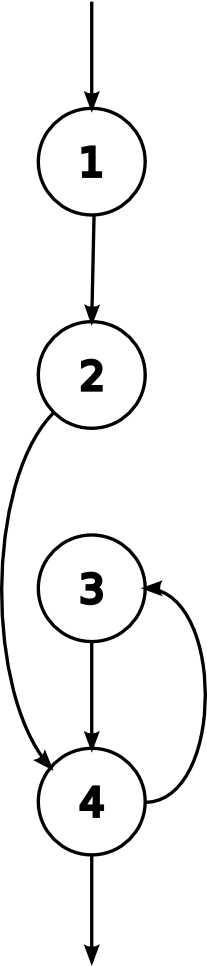
\includegraphics{figs/QuickSortMain.png}}
\caption{\label{QuickSortMain}Loop in the `Main' method of quick-sort}
\end{figure}

\subsubsection{Finding loops and conditionals}
       \impref{Finding loops}

Loops are found by repeatedly applying the T1-T2 transformations.
In this case the first transformation to be performed will be
a T2 transformation on basic blocks 1 and 2.
This will result in this `tree':

\begin{verbatim}
// AcyclicGraph 10 (Successors:4 Parent:0)
AcyclicGraph_10:
{
    // BasicBlock 1 (Successors:2 Parent:10)
    BasicBlock_1:
    int[] V_0 = new int[args.Length];
    int i = 0;
    goto BasicBlock_2;
    
    // BasicBlock 2 (Predecessors:1 Parent:10)
    BasicBlock_2:
    goto BasicBlock_4;
    
}

// BasicBlock 3 (Predecessors:4 Successors:4 Parent:0)
BasicBlock_3:
V_0[i] = Int32.Parse(args[i]);
i++;
goto BasicBlock_4;

// BasicBlock 4 (Predecessors:3,10 Successors:5,3 Parent:0)
BasicBlock_4:
if (i < V_0.Length) goto BasicBlock_3; 
goto BasicBlock_5;
\end{verbatim}

Note how the links changed.  Basic blocks 1 and 2 are now considered as a 
single node 10 -- the predecessor of basic block 4 is now 10 rather then 2.
Links within the node 10 are limited just to the scope of that node.

Several further transformations are performed until all loops are found.

Conditional statements are identified as well.  
This code has one conditional statement which 
does not have any code in the bodies other then the \verb|goto|s.

\newpage

\begin{verbatim}
// BasicBlock 1 (Successors:2 Parent:0)
BasicBlock_1:
int[] V_0 = new int[args.Length];
int i = 0;
goto BasicBlock_2;

// BasicBlock 2 (Predecessors:1 Successors:11 Parent:0)
BasicBlock_2:
goto BasicBlock_4;

// Loop 11 (Predecessors:2 Successors:5 Parent:0)
Loop_11:
for (;;) {
    // ConditionalNode 22 (Predecessors:3 Successors:3 Parent:11)
    ConditionalNode_22:
    BasicBlock_4:
    if (i >= V_0.Length) {
        goto BasicBlock_5;
        // Block 21 (Parent:22)
        Block_21:
    
    } else {
        goto BasicBlock_3;
        // Block 20 (Parent:22)
        Block_20:
    
    }
    
    // BasicBlock 3 (Predecessors:22 Successors:22 Parent:11)
    BasicBlock_3:
    V_0[i] = Int32.Parse(args[i]);
    i++;
    goto BasicBlock_4;
    
}
\end{verbatim}

\subsubsection{Final version}

Let us see the code once again without the comments and empty lines.

\begin{verbatim}
BasicBlock_1:
int[] V_0 = new int[args.Length];
int i = 0;
goto BasicBlock_2;
BasicBlock_2:
goto BasicBlock_4;
Loop_11:
for (;;) {
    ConditionalNode_22:
    BasicBlock_4:
    if (i >= V_0.Length) {
        goto BasicBlock_5;
        Block_21:
    } else {
        goto BasicBlock_3;
        Block_20:
    }
    BasicBlock_3:
    V_0[i] = Int32.Parse(args[i]);
    i++;
    goto BasicBlock_4;
}
\end{verbatim}

\newpage
\subsection{Abstract Syntax Tree representation (part 2)}
\subsubsection{Removal of `goto' statements}
       \impref{Removal of `goto' statements}

All of the \verb|goto| statements in the code above can be 
removed or replaced.  After the removal of \verb|goto| statements
we get the following much simpler code:

\begin{verbatim}
int[] V_0 = new int[args.Length];
int i = 0;
for (;;) {
    if (i >= V_0.Length) {
        break;
    }
    V_0[i] = Int32.Parse(args[i]);
    i++;
}
\end{verbatim}

Note that the `false' body of the \verb|if| statement was removed
because it was empty.

\subsubsection{Simplifying loops}
       \impref{Simplifying loops}

The code can be further simplified by pushing the loop initializer,
condition and iterator inside the \verb|for(;;)|:

\begin{verbatim}
int[] V_0 = new int[args.Length];
for (int i = 0; i < V_0.Length; i++) {
    V_0[i] = Int32.Parse(args[i]);
}
\end{verbatim}

This concludes the decompilation of quick-sort.

\clearpage

{\vspace*{60mm} \centering This page is intentionally left blank\\ Please turn over \newpage}


\subsection{Original quick-sort (complete source code)}
\label{Original quick-sort}
\lstinputlisting[basicstyle=\footnotesize]
{./figs/QuickSort_original.cs}

\newpage

\subsection{Decompiled quick-sort (complete source code)}
\label{Decompiled quick-sort}
\lstinputlisting[basicstyle=\footnotesize]
{./figs/10_Short_type_names_2.cs}


\section{Advanced and unsupported features}

This section demonstrates decompilation of more advanced application. 
The examples that follow were produced by decompiling a reversi game%
\footnote{Taken from the CodeProject.  Written by Mike Hall.}.

The examples demonstrate advanced features of the decompiler
and in some cases its limitations (i.e.\ still unimplemented features).




\subsection{Properties and fields}

Properties and fields are well-supported.

\emph{Original:}
\begin{verbatim}
private int[,] squares;
private bool[,] safeDiscs;

public int BlackCount {
  get { return blackCount; }
}
public int WhiteCount {
  get { return whiteCount; }
}
\end{verbatim}

\emph{Decompiled:}
\begin{verbatim}
private System.Int32[,] squares;
private System.Boolean[,] safeDiscs;

public int BlackCount {
    get { return blackCount; }
}
public int WhiteCount {
    get { return whiteCount; }
}
\end{verbatim}

The decompiled code is correct.

The type \verb|System.Int32[,]| was not simplified to \verb|int[,]|.




\subsection{Short-circuit boolean expressions}

\emph{Original:}
\begin{verbatim}
if (r < 0 || r > 7 || c < 0 || c > 7 ||
    (r - dr == row && c - dc == col) ||
    this.squares[r, c] != color)
  return false;
\end{verbatim}

\emph{Decompiled:}
\begin{verbatim}
if (i < 0 || i > 7 || j < 0 || j > 7 ||
    i - dr == row && j - dc == col ||
    squares[i, j] != color) {
      return false;
}
\end{verbatim}


The decompiled code is correct.  Variable names were lost during compilation.
By precedence rules it was possible to remove the parenthesis.




\subsection{Short-circuit boolean expressions 2}

\emph{Original:}
\begin{verbatim}
if ((hasSpaceSide1  && hasSpaceSide2 ) ||
    (hasSpaceSide1  && hasUnsafeSide2) ||
    (hasUnsafeSide1 && hasSpaceSide2 ))
  return true;
\end{verbatim}

\emph{Decompiled:}
\begin{verbatim}
if (flag && flag2 || flag && flag4 || flag3 && flag2) {
  return true;
}
\end{verbatim}

The decompiled code is correct.  Variable names were lost during compilation.



\subsection{Complex control nesting}

\emph{Original:}
\begin{verbatim}
bool statusChanged = true;
while (statusChanged)
{
  statusChanged = false;
  for (i = 0; i < 8; i++)
    for (j = 0; j < 8; j++)
      if (this.squares[i, j] != Board.Empty &&
         !this.safeDiscs[i, j] && 
         !this.IsOutflankable(i, j)) {
            this.safeDiscs[i, j] = true;
            statusChanged = true;
      }
}
\end{verbatim}

\emph{Decompiled:}
\begin{verbatim}
for (bool flag = true; flag;) {
  flag = false;
  for (int i = 0; i < 8; i++) {
    for (int j = 0; j < 8; j++) {
      if (squares[i, j] != Empty &&
         !safeDiscs[i, j] &&
         !IsOutflankable(i, j)) {
            safeDiscs[i, j] = true;
            flag = true;
       }
    }
  }
}
\end{verbatim}

The decompiled code is correct.

A \verb|for| loop was used instead of \verb|while| loop.
The decompiler always uses \verb|for| loop.

In the example, four control structures are nested;
even more levels do not cause any problems.





\subsection{Multidimensional arrays}

Multidimensional arrays are supported.

\emph{Original:}
\begin{verbatim}
this.squares = new int[8, 8];
this.safeDiscs = new bool[8, 8];
// Clear the board and map.
int i, j;
for (i = 0; i < 8; i++)
  for (j = 0; j < 8; j++) {
    this.squares[i, j] = Board.Empty;
    this.safeDiscs[i, j] = false;
  }
\end{verbatim}

\emph{Decompiled:}
\begin{verbatim}
squares = new int[8, 8];
safeDiscs = new bool[8, 8];
for (int i = 0; i < 8; i++) {
  for (int j = 0; j < 8; j++) {
    squares[i, j] = Empty;
    safeDiscs[i, j] = false;
  }
}
\end{verbatim}

The decompiled code is correct and even slightly simplified.





\subsection{Dispose method}

This is the standard .NET dispose method for a form.

\emph{Original:}
\begin{verbatim}
if(disposing) {
  if (components != null) {
    components.Dispose();
  }
}
\end{verbatim}

\emph{Decompiled:}
\begin{verbatim}
if (disposing && components) {
  components.Dispose();
}
\end{verbatim}

The decompiler did a good job identify that the two
\verb|if|s can be expressed as short-circuit expression.

On the hand, it failed to distinguish being `true' and being `non-null'
-- on the bytecode level these are the same thing (together with being `non-zero').




\subsection{Event handlers}

Event handlers are not supported.

\emph{Original:}
\begin{verbatim}
this.aboutMenuItem.Click +=
  new System.EventHandler(this.aboutMenuItem_Click);
\end{verbatim}

\emph{Decompiled:}
\begin{verbatim}
aboutMenuItem.add_Click(
  new System.EventHandler(this, IL__ldftn(aboutMenuItem_Click()))
);
\end{verbatim}

Note how the unsupported bytecode \verb|ldftn| is presented.



\subsection{Constructors}

\emph{Original:}
\begin{verbatim}
this.infoPanel.Location = new System.Drawing.Point(296, 32);
\end{verbatim}

\emph{Decompiled:}
\begin{verbatim}
infoPanel.Location = new System.Drawing.Point(296, 32);
\end{verbatim}

The decompiled code is correct including the constructor arguments.


\subsection{Property access}

\emph{Original:}
\begin{verbatim}
this.infoPanel.Name = "infoPanel";
\end{verbatim}

\emph{Decompiled:}
\begin{verbatim}
infoPanel.Name = "infoPanel";
\end{verbatim}

The decompiled code is correct.

Note that properties are actually set methods.  This is,
\verb|set_Name(string)| here. 


\subsection{Object casting}

\emph{Original:}
\begin{verbatim}
this.Icon = ((System.Drawing.Icon)(resources.GetObject("$this.Icon")));
\end{verbatim}

\emph{Decompiled:}
\begin{verbatim}
Icon = (System.Drawing.Icon)V_0.GetObject("$this.Icon");
\end{verbatim}

The decompiled code is correct.



\subsection{Boolean values}

In the .NET Runtime there is no difference between
integers and booleans.  Handling of this is delicate.

\emph{Original:}
\begin{verbatim}
return false;
\end{verbatim}

\emph{Decompiled:}
\begin{verbatim}
return false;
\end{verbatim}

The decompiled code is correct.

\emph{Original:}
\begin{verbatim}
this.infoPanel.ResumeLayout(false);
\end{verbatim}

\emph{Decompiled:}
\begin{verbatim}
infoPanel.ResumeLayout(0);
\end{verbatim}

This code is incorrect -- the case where boolean is
passed as argument still has no been considered in the decompiler.
This is just case-by-case laborious work.



\subsection{The `dup' instruction}

The \verb|dup| instruction is handled well.

\emph{Decompiled: (`dup' unsupported)}
\begin{verbatim}
expr175 = this;
expr175.whiteCount = expr175.whiteCount + 1;
\end{verbatim}

\emph{Decompiled: (`dup' supported)}
\begin{verbatim}
whiteCount++;
\end{verbatim}


% coverage for a typical binaries (I like that one :-) )
% Anonymous methods, Enumerators, LINQ

%%%%%%%%%%%%%%%%%%%%%%%%%%%%%%%%%%%%%%%%%%%%%%%%%%%%%%%%%%%%%%%%%%%%%%%%%%%%%%%
% 2 Page
\cleardoublepage
\chapter{Conclusion}

The project was a success.
The goal of the project was to decompile an implementation
of a quick-sort algorithm and this goal was achieved well.
The C\# source code produced by the decompiler is
virtually identical to the original source code%
\footnote{See pages \pageref{Original quick-sort} and \pageref{Decompiled quick-sort} in the evaluation chapter.}.
In particular, the source code compiles back to identical .NET CLR code.

More complex programs than the quick-sort implementation 
were considered and the decompiler was improved to handle them better.
The improvements include:
\begin{itemize}
	\item Better support for several bytecodes related to:
	creation and casting of objects, multidimensional arrays,
	virtual method invocation, property access and field access.
	\item Support for the \verb|dup| bytecode which does not
	occur very frequently in programs.  In particular, it does not
	occur in the quick-sort implementation.
	\item Arbitrarily complicated short-circuit boolean expression
	are handled.  Furthermore, both the short-circuit
	and the traditional boolean expressions are simplified
	using rules of logic (e.g.\ using De Morgan's laws).
	\item Nested high-level control structures are handled
	well (e.g.\ nested loops).
	\item The performance is improved by using basic blocks.
	\item The removal of \verb|goto|s was improved to work
	in almost any scenario (by using the `simulator' approach).
\end{itemize}


\section{Hindsight}

I am very satisfied with the current implementation.
Whenever I have seen an opportunity for improvement,
I have have refactored the code right away.
As a result of this, I think that the algorithms and data structures 
currently used are very well suited for the purpose.

If I were to reimplement the project, I would merely
save time by making the right design decisions right away.

Here are some issues that I have encountered are resolved:

\begin{itemize}
	\item During the preparation phase, I have spend reasonable
	amount of time researching algorithms for finding of loops.
	I found most of the algorithms either unintuitive or not
	not sufficiently robust for all scenarios.
	Therefore, I have derived my own algorithm based on the
	T1-T2 transformations.
	\item I have initially used the \emph{CodeDom} library
	for the abstract syntax tree.  
	In the end, \emph{NRefactory} proved much more suitable.
%	\item I have initially directly used the objects provided by
%	\emph{Cecil} library as the first code representation.
%	Making an own copy turned out to be better since the objects
%	could be more easily manipulated and annotated.
	\item I have eventually made the stack-based and
	variable-based code representations quite distinct and
	decoupled.  This allowed greater freedom for transformations.
	\item Initially the links between nodes were manually kept
	in synchronization during transformations.
	It is more convenient and robust just to throw the links away
	and recalculate them.
	\item The removal of \verb|goto|s was gradually pushed
	all the way to the last stage of decompilation where it is
	most powerful and safest.
\end{itemize}

\section{Future work}

The theoretical problems have been resolved.
However, a lot of laborious work still needs to be done before
the decompiler will be able to handle all .NET executables.

The decompiler could be extended to recover C\# compile-time
features like anonymous methods, enumerators or LINQ expressions.

The decompiler greatly overlaps with a verification of .NET executables
(the code needs to be valid in order to be decompiled).
The project could be forked to create .NET verifier.

I am the primary developer of the SharpDevelop debugger.
I would like integrate the decompiler with the debugger so
that is it possible to debug applications with no source code.


%%%%%%%%%%%%%%%%%%%%%%%%%%%%%%%%%%%%%%%%%%%%%%%%%%%%%%%%%%%%%%%%%%%%%%%%%%%%%%%
\cleardoublepage
\chapter{Project Proposal}
%\thispagestyle{empty}

%\rightline{\large\emph{David Srbeck\'y}}
%\medskip
%\rightline{\large\emph{Jesus College}}
%\medskip
%\rightline{\large\emph{ds417}}

\vfil
\vspace{0.4in}
\centerline{\large Part II of the Computer Science Project Proposal}
\vspace{0.4in}
\centerline{\Large\bf .NET Decompiler}
\vspace{0.3in}
\centerline{\large\emph{October~14,~2007}}

\vfil

{\bf Project Originator:} \emph{David Srbeck\'y}

\vspace{0.1in}

{\bf Resources Required:} See attached Project Resource Form

\vspace{0.3in}

{\bf Project Supervisor:} \emph{Alan Mycroft}

\vspace{0.3in}

{\bf Director of Studies:} \emph{Jean Bacon} and \emph{David Ingram}

\vspace{0.3in}

{\bf Overseers:} \emph{Anuj Dawar} and \emph{Andrew Moore}

\vfil
\eject

\section*{Introduction and Description of the Work}
The \emph{.NET Framework} is a general-purpose software development platform 
which is very similar to \emph{Java}.  It includes extensive class library 
and, similarly to Java, is based on the virtual machine model.  The executable 
code for a \emph{.NET} program is stored in a file called \emph{assembly} 
which consists of class metadata and a stack-based bytecode called Common 
Intermediate Language (\emph{CIL} or \emph{IL}).

In general, any programming language can be compiled to \emph{.NET} and 
there are dozens of compilers that compile into \emph{CIL}.  The most 
common language used for \emph{.NET} development is \emph{C\#}.

The goal of this project is to decompile \emph{.NET} assemblies back into 
equivalent \emph{C\#} source code.  Compared to decompilation of 
conventional assembly code, this task is hugely simplified by the 
presence of metadata in the \emph{.NET} assemblies.  The metadata contains 
complete information about classes, methods and fields.  The method bodies 
consist of stack-based \emph{IL} code which needs to be decompiled into 
higher-level \emph{C\#} statements.  Data-flow analysis will need to be 
employed to transform the stack-based data model into one that uses 
temporary local variables and composition of expressions.  Control-flow 
analysis will be used to recreate high level control structures like 
\verb|for| loops and conditional branching.

\section*{Resources Required}
\begin{itemize}
	\item{\textbf{My own machine}\\
		(1.6 GHz CPU, 1.5 GB of RAM, 50 GB \& 75 GB Disks, 
		Windows XP SP2 OS) \\
		Used for development
	}
	\item{\textbf{Student-Run Computing Facility (SRCF)}\\
		Used for running the \emph{SVN} server
	}
	\item{\textbf{Public Workstation Facility (PWF)}\\
		Used for storage of back-ups
	}
\end{itemize}

\newpage

\section*{Starting Point}
I plan to implement the project in \emph{C\#}.  I have been using this 
language for over five years now and so I do not have to spend any time 
learning a new language.  It also means that I will not be having any 
problems neither with the syntax of the language nor with any peculiar 
error messages produced by the compiler or by the runtime.

I have written an integrated \emph{.NET} debugger for the 
\emph{SharpDevelop} IDE.  During that I have obtained some basic knowledge 
about metadata and lower-level functionality in \emph{.NET}.  I can read 
\emph{.NET} bytecode and, with the help of reference manual, I can write 
short programs in it.

The metadata and bytecode needs to be read form the assembly files. 
I plan to use the \emph{Cecil} library for it.  I am not familiar with this 
library, but I do not expect to have any difficulties with it.

\section*{Substance and Structure of the Project}
The project consists of the following major work items:
\begin{enumerate}
\newcommand{\milestone}[1]{\item \textbf{#1} \\}

\milestone{Preliminary research}
I will have to research the following topics:
\begin{itemize}
	\item {\emph{Cecil} library}
		- \emph{Cecil} is the library which I will use for reading of the 
		metadata.  It will need to get familiar with its public API.
		Because it is open-source, it might be valuable to get some basic 
		understanding of its source code as well.
	\item {\emph{CIL} bytecode}
		- The runtime of the \emph{.NET Framework} is described in 
		ECMA-335 Standard: \emph{``CLI Specification -- Virtual Machine''} 
		(556 pages).  I will need to get familiar with this document since 
		I will be using it as the main reference.  I will be especially 
		interested in \emph{Partition III -- CIL Instruction Set}.
	\item {Decompilation theory} - I will need to get familiar with the 
		theory behind decompilation of programs.  Cristina Cifuentes' 
		PhD thesis \emph{``Reverse Compilation Techniques''} might prove as 
		especially useful starting point.
\end{itemize}

The research of these topics should not be too extensive.  I only indeed to 
get sufficient background knowledge in these areas and then return to the 
finner details when I needed them.

\milestone{Create a skeleton of the code}
It will be necessary to read the assembly metadata and create a \emph{C\#} 
source code that has the same classes, fields and methods.  The method 
signatures have to match the ones in the assembly.  At this point the method 
bodies can be left empty.

\milestone{Read and disassemble \emph{.NET} bytecode}
The next step is to read the bytecode for each method, disassemble it and 
output it as comments (for example, \verb|// IL_01: ldstr "Hello world"|).  
This will help me learn how to use the \emph{Cecil} library to read the 
bytecode and how to process it.  I also expect that this output will be 
extremely helpful for debugging purposes later on.

\milestone{Start creating r-value expressions}
Ignoring the stack of the virtual machine, some bytecodes can be 
straightforwardly converted into expressions.  For example:
\begin{verbatim}
ldstr "Hello world"      - string "Hello world"
ldnull                   - 'null' reference
ldc.i4.0                 - 4 byte integer of value 0
ldc.i4 123               - 4 byte integer of value 123
ldarg.0                  - the first method argument
ldloc.0                  - the first local variable in the method
\end{verbatim}

The goal of this stage is to create \emph{C\#} expressions for several of 
the most important bytecodes.

Function calls and arithmetic operations are also expressions, but at this 
stage I do not know their inputs and so I will have to use dummy values as 
their inputs.

\milestone{Conditional and unconditional branching}
There are several bytecodes that investigate one or two values on the top 
of stack and then, if a given condition is met, branch to different 
location.  (\verb|br|, \verb|brfalse|, \verb|brtrue|, \verb|beq|, 
\verb|bge|, \verb|bgt|, etc...)

The goal of this stage is to use \emph{C\#} labels and \verb|goto|
statements to recreate this flow of control.  (eg translate 
\verb|brfalse IL_02| to \verb|if (input == false) goto Label_02;|)

As in the previous stage the inputs (ie the values at the top of stack) are
still not know.

\milestone{Simple data-flow analysis}
This is where it begins to be difficult.  Consider the code:
\begin{verbatim}
// Load "Hello, world!" on top of the stack
IL_01: ldstr "Hello, world!"
// Print the top of the stack to the console
IL_02: call void [mscorlib]System.Console::WriteLine(string)
\end{verbatim}
Both of these are already decompiled as expressions, however the call 
has a dummy value as its argument.  The goal of this stage is to perform 
as simple data-flow analysis as possible.  The text "Hello, world!" must 
find its way to the method call.  At this point it will probably be through 
one or even two temporary variables.  For example:
\begin{verbatim}
String il_01_expression = "Hello, world!";
String il_02_argument_1 = il_01_expression;
System.Console.WriteLine(il_02_argument_1);
\end{verbatim}
The most difficult part will be handling of control flow.  Different values 
can be on stack depending on which branch of code was executed.  At this 
stage it will be necessary to create and analyse control flow graph.  As a 
result of this stage, many temporary variables might be introduced to the 
code.

\milestone{Round-trip quick-sort algorithm}
At this point very simple applications should probably successfully 
decompile and compile again (round-trip).

The goal of this stage is to fix bugs and to add features so that simple 
algorithm like quick-sort can be successfully round-tripped without need to 
manually change the produced \emph{C\#} source code.  At this point there is 
no restriction on the aesthetics of the source code.  The only requirement 
is that it does compile. 

There are many features of \emph{.NET} that I do not plan to support at 
this point.  For example, boxing \& unboxing, casting, generics and 
exception handling.  In general, all non-essential features are excluded.

\milestone{Further data-flow analysis}
Employ more advanced data-flow analysis to simplify the generated \emph{C\#} 
code.  Many temporary variables can be probably removed, relocated or 
renamed according to their use.

\emph{[This task has variable scope and if the project starts falling behind 
schedule, simpler algorithms can be employed and vice versa.]}

\milestone{Control-flow analysis}
The goal of this stage is to use control-flow analysis to regenerate 
high-level structures like \verb|if| statements and \verb|for| loops. 
It will not be possible to eliminated all \verb|goto| statements, but they 
should be avoided whenever possible.

\emph{[This task has variable scope and if the project starts falling behind 
schedule, simpler algorithms can be employed and vice versa.]}

\milestone{Assembly resources}
\emph{.NET} assemblies can have files embed in them.  These files can then 
be accessed at runtime and thus the programs might require them.

The goal is to extract the resources so that they can be included during 
the recompilation process.

\emph{[Optional.  This is an optional goal which will be done only if the 
project development goes much better then originally anticipated.]}

\milestone{Advanced features}
Add commonly used features which where ignored so far - for example, 
boxing \& unboxing, casting, generics and exception handling.

\emph{[Optional.  This is an optional goal which will be done only if the 
project development goes much better then originally anticipated.]}

\milestone{Round-trip Mono}
The ultimate goal of this project is to be able to round-trip any 
\emph{.NET} assembly.  This means that for any given assembly the 
Decompiler should produce \emph{C\#} source code which is valid (does 
compile again without error).  Even more importantly, the program produced 
by the compilation of the source code should be semantically same as the 
original one.  Since the bytecode will in general differ, this condition is 
difficult to verify.  One way to check that the Decompiler preserves the 
meaning of programs is to simply try it.

\emph{Mono} is open-source reimplantation of the \emph{.NET Framework}.
The major part of it are the \emph{.NET} class libraries which can be 
used for testing of the Decompiler.  The project is open-source and so if 
any decompilation problems occur, it is possible to investigate the 
source code of these libraries.  Furthermore, the libraries come with 
extensive unit testing suite so it is possible to verify that the 
round-tripped libraries are not broken.

The goal of this final stage is to successfully round-trip all \emph{Mono} 
libraries and pass the unit tests.  This would probably involve enormous 
amount of bugfixing, investigation and handling of corner cases.  All 
remaining \emph{.NET} features would have to be implemented.

\emph{[Optional.  This last stage is huge and impossible to be finished 
within the time frame of Part II project.  If all goes well, I expect 
that it will take at least one more year for the project to mature to 
this point.]}

\milestone{Write the dissertation}
The last and most important piece of work is to write the dissertation.
Being a non-native English speaker, I expect this to take considerable
amount of time.  I plan to spend the last seven weeks of project time
on it.  This includes the end of Lent Term and the whole Easter vacation.
I plan to have the dissertation finished by the start of Easter term.

\end{enumerate}

\newpage

\section*{Success Criteria}
The Decompiler should successfully round-trip a quick-sort algorithm 
(or any algorithm of comparable complexity). 
That is, when an assembly containing the algorithm is 
decompiled, the produced \emph{C\#} source code should be both 
syntactically and semantically correct.  The bytecode produced
by compilation of the generated source code is not expected to be
identical to the original one, but it is expected to be equivalent.
That is, the binary may be different but it still needs to be a correct 
implementation of the algorithm.

To achieve this the Decompiler will need to have the following features:
\begin{itemize}
	\item Handle integers and integer arithmetic
	\item Create and be able to use integer arrays
	\item Branching must be successfully decompiled
	\item Several methods can be defined
	\item Methods can have arguments and return values
	\item Methods can be called recursively
	\item Integer command line arguments can be read and parsed
	\item Text can be outputted to the standard console output
\end{itemize}

See the following page for a \emph{C\#} implementation of a quick-sort
algorithm which will be used to demonstrate successful implementation
of these features.

I plan to achieve the success criteria by the progress report dead-line 
and then spend the rest of the time available by increasing the quality 
of the generated source code  (ie ``Further data-flow analysis'' and 
``Control-flow analysis'').


\newpage

{
\linespread{0.90}
\lstinputlisting[
  basicstyle=\footnotesize,
  language={[Sharp]C},
  tabsize=4,
  numbers=left,
  frame=single,
  title=Quick-sort algorithm
]{
  ../../tests/QuickSort/Program.cs
}
}
\newpage
\section*{Timetable and Milestones}
The work shall start on the Monday 22.10.2007 and is expected to 
take 20 weeks in total.

\vspace{0.1in}
\newcommand{\milestone}[3]{\emph{#1} & \emph{#2} & \textbf{#3} \\}
\begin{tabular}{l l l}
	\milestone{22 Oct - 28 Oct}{(week  1)}{Preliminary research}
	\milestone{29 Oct -  4 Nov}{(week  2)}{Create a skeleton of the code}
	\milestone{5 Nov  - 11 Nov}{(week  3)}{Read and disassemble \emph{.NET} bytecode}
	\milestone{12 Nov - 18 Nov}{(week  4)}{Start creating r-value expressions}
	\milestone{19 Nov - 25 Nov}{(week  5)}{Conditional and unconditional branching}
	\milestone{26 Nov -  9 Dec}{(weeks 6 and 7)}{Simple data-flow analysis}
	\milestone{10 Dec - 20 Jan}{}{\textnormal{Christmas vacation}}
	\milestone{21 Jan - 27 Jan}{(week  8)}{Round-trip quick-sort algorithm}
	\milestone{26 Jan - 27 Jan}{}{Write the Progress Report}
	\milestone{28 Jan - 10 Feb}{(weeks 9 and 10)}{Further data-flow analysis}
	\milestone{11 Feb -  2 Mar}{(weeks 11 to 13)}{Control-flow analysis}
	\milestone{3 Mar  - 20 Apr}{(weeks 14 to 20)}{Write the dissertation \textnormal{(over Easter vacation)}}
	\milestone{21 Apr onwards }{}{\textnormal{Easter term -- Preparation for exams}}
\end{tabular}
\vspace{0.1in}

Unscheduled tasks: \textbf{Assembly resources}; \textbf{Advanced features};
 \textbf{Round-trip Mono}


\end{document}
